
\documentclass[11pt]{book}
% Basic document setup
\usepackage[a4paper,margin=1in]{geometry}
\usepackage[latin]{babel}
\usepackage{graphicx}
\usepackage{booktabs}
\usepackage{epstopdf}
\usepackage{float}
\usepackage{tikz}
\usepackage{pgfplots}
\usepackage{pgffor}
\usepackage{enumitem}
\usepackage{tabularx}
\usepackage{graphicx}
\usepackage{changepage}
\usepackage{verbatim}
\usepackage{setspace}
\usepackage{ragged2e}
\usepackage{array}
\usepackage{pgffor} % Required for \foreach
\usepackage{ifoddpage}
\usepackage{catchfile} 
\usepackage{xstring}
\usepackage[most]{tcolorbox}  % Ensure this is included in your preamble
\usepackage{array}
\usepackage{colortbl}
\usepackage{caption}
\usepackage{varwidth}
\usepackage{pagecolor}
\usepackage{lipsum} % optional for filler text



\pgfplotsset{compat=1.18}

% Typography and text formatting
\usepackage[protrusion=true,expansion=true]{microtype}
\usepackage{CJK}
\newcommand{\katakana}[1]{\begin{CJK}{UTF8}{min}#1\end{CJK}}
\usepackage{shadowtext}
\usepackage{bbding}
\usepackage{textcomp}
\usepackage{hyperref}
\usepackage{parskip}
\usepackage{multicol}
\usepackage{needspace}
\usepackage{etoolbox}
\usepackage{pifont}  % for nice symbols like the filled circle

% Math packages
\usepackage{amsmath, amssymb, physics}
\usepackage{unicode-math}

% Multilingual support
\usepackage{polyglossia}
\usepackage{amsfonts}
\usepackage{lmodern} 
\setdefaultlanguage{english}
\setotherlanguage{greek}
\setotherlanguage{hebrew}
\setotherlanguage{sanskrit}

% Font configuration
\usepackage{fontspec}
\setmainfont{Libertinus Serif}                    % Main serif font
\newfontfamily\historyfont{Crimson Pro}           % Historical section font
          % Technical section font
\newfontfamily\commentaryfont{Crimson Pro}        % Commentary font
\newfontfamily\greekfont[Script=Greek]{Linux Libertine O}
\newfontfamily\hebrewfont[Script=Hebrew]{Ezra SIL}
\newfontfamily\sanskritfont[Script=Devanagari]{Noto Sans Devanagari}
\newfontfamily\piefont{Charis SIL}
\newfontfamily\ipafont{Charis SIL}

\newfontfamily\summaryfont{Libertinus Serif Italic} % Summary font
\newfontfamily\technicalfont[ItalicFont={XITS Math}]{XITS Math}

% Color definitions
\usepackage{xcolor}
\definecolor{historycolor}{RGB}{70,30,0}         % Warm brown for historical sections
\definecolor{technicalcolor}{RGB}{0,20,60}       % Deep blue for technical sections
\definecolor{commentarycolor}{RGB}{0,0,0}        % Black for commentary
\definecolor{summarycolor}{RGB}{90,90,90}        % Gray for summaries
\definecolor{linkcolor}{RGB}{0,85,155}           % Link color for hyperlinks
\definecolor{SUMMARYCOLOR}{RGB}{90,90,90}        % Gray for summaries (uppercase)
\definecolor{lavender}{RGB}{248,243,255}\definecolor{lavender}{RGB}{230,230,250}
\definecolor{lightgray}{gray}{0.85}


% Section styling with titlesec
\usepackage{titlesec}
\usepackage{tocloft}  % For customizing TOC

\titleformat{\chapter}[hang]
    {\normalfont\huge\bfseries}{\thechapter}{1em}{} % Chapter title styling
\titlespacing*{\chapter}{0pt}{0pt}{10pt}            % Adjust spacing around chapters
\titleformat{\section}[hang]
    {\normalfont\Large\bfseries}{\thesection}{1em}{} % Section title styling
\titlespacing*{\section}{0pt}{10pt}{5pt}             % Adjust spacing around sections

% Frame and box packages
\usepackage[framemethod=TikZ,skipabove=6pt,skipbelow=6pt]{mdframed}
\usetikzlibrary{decorations.pathmorphing, decorations.shapes, decorations.footprints, shapes.geometric, positioning, patterns, fit,arrows.meta, decorations.pathmorphing, backgrounds, calc, decorations.fractals}
\mdfsetup{splitbottomskip=2pt, splittopskip=2pt}

\usetikzlibrary{lindenmayersystems}

% Spacing and layout settings
\setlength{\parindent}{0pt}      % No paragraph indentation
\setlength{\parskip}{0.5em}      % Paragraph spacing for better readability
\setlength{\columnsep}{15pt}     % Adjust column separation for multicol layout


% Force content to start on the next even-numbered page

\newcommand{\startchapter}{%
  \clearpage
  \checkoddpage
  \ifoddpage
    % already odd — do nothing
  \else
    \hbox{}
    \thispagestyle{empty}
    \clearpage
  \fi
}




% TOC customization for chapter summaries
\setlength{\cftbeforechapskip}{1.0em}  % Increase space between TOC entries
\setlength{\cftchapindent}{0em}        % Chapter indent in TOC
\renewcommand{\cftchapfont}{\bfseries} % Chapter font in TOC

% Header setup with fancyhdr - MUST be loaded after titlesec
\usepackage{fancyhdr}
\setlength{\headheight}{14pt}  % Slightly more than the required 13.59999pt

% Create chapter title extraction command to handle only the title part
\makeatletter
\def\extracttitle#1\\#2\@nil{#1}
\makeatother

% Define the main page style
\pagestyle{fancy}
\fancyhf{} % Clear all header and footer fields
\fancyhead[LE,RO]{\thepage}
\fancyhead[RE]{\textit{\leftmark}}
\fancyhead[LO]{\textit{\rightmark}}
\renewcommand{\headrulewidth}{0.4pt}
\renewcommand{\footrulewidth}{0pt}

% Fix the chapter page style (first page of each chapter)
\fancypagestyle{plain}{%
  \fancyhf{} % Clear all header and footer fields
  \fancyfoot[C]{\thepage} % Just page number at bottom
  \renewcommand{\headrulewidth}{0pt} % No header rule on first page
}

% Modify chaptermark to extract just the title
% Better approach to handle headers without the summary
\makeatletter
% Simple approach - standard chapter marking
\renewcommand{\chaptermark}[1]{%
  \markboth{\MakeUppercase{\chaptername\ \thechapter.\ #1}}{}}
\renewcommand{\sectionmark}[1]{\markright{\thesection.\ #1}}

% Helpers to input title and summary from file
\newcommand{\inputtitle}[1]{\IfFileExists{#1/title.tex}{An Axiom of Your Choice
}{MissingTitle}}
\newcommand{\inputsummary}[1]{\IfFileExists{#1/summary.tex}{Fireflies produce light through a precise biochemical reaction where luciferase enzymes catalyze the oxidation of luciferin in specialized abdominal photocytes. This process converts chemical energy to light with remarkable efficiency — over 80\% compared to an incandescent bulb's 5\% — creating "cold light" with minimal heat production. Fireflies control flash patterns by regulating oxygen flow through tracheal networks, producing species-specific signals that prevent cross-species mating attempts. The light emission peaks in the yellow-green spectrum (560-590 nm), optimized for visibility in low-light conditions. Reflective layers of uric acid crystals direct photons outward, enhancing visibility. This natural system demonstrates the convergence of genetics, biochemistry, cellular biology, and quantum physics, where electron transitions between energy levels determine the wavelength of emitted photons.
}{MissingSummary}}

\newtcolorbox{shadedstory}[1][]{
  colback=gray!10,
  colframe=gray!50,
  sharp corners,
  boxrule=0.8pt,
  left=10pt,
  right=10pt,
  top=10pt,
  bottom=10pt,
  title=#1,
  fonttitle=\bfseries\large,
  enhanced,
}



\newcommand{\chapterseparator}{%
  \begin{center}
    \begin{tikzpicture}[baseline]

      % Left-growing fractal
      \begin{scope}[xscale=-1, shift={(-2cm,0)}]
        \draw[gray!70!black, thick,
          l-system={
            rule set={F -> FF-[-F+F]+[+F-F]},
            axiom=F,
            order=4,
            step=2pt,
            randomize step percent=35,
            angle=30,
            randomize angle percent=10
          }]
          lindenmayer system;
      \end{scope}

      % Right-growing fractal
      \begin{scope}[shift={(2cm,0)}]
        \draw[gray!70!black, thick,
          l-system={
            rule set={F -> FF-[-F+F]+[+F-F]},
            axiom=F,
            order=4,
            step=2pt,
            randomize step percent=35,
            angle=30,
            randomize angle percent=10
          }]
          lindenmayer system;
      \end{scope}

    \end{tikzpicture}
  \end{center}
}





% Custom chapter with summary command (TOC only, no visible title)
\newcommand{\chapterwithsummary}[3][]{%
  % #1 = optional label
  % #2 = chapter title
  % #3 = chapter summary

  % TOC entry only (multi-line)
  \addcontentsline{toc}{chapter}{%
    \protect\numberline{\thechapter}#2\\
    {\normalfont\small\textit{\textcolor{summarycolor}{#3}}}%
  }

  % Update header with title only (no page title)
  \chaptermark{#2}%

  % Apply label if provided
  \ifx\\#1\\\else\label{#1}\fi

  % Avoid rendering a visible chapter heading
  \phantomsection % for correct link targets
  \vspace*{-3em} % suppress visual whitespace
}


\newread\file
\newcommand{\readfirstline}[2]{%
  \openin\file=#2
  \read\file to \temp
  \closein\file
  \xdef#1{\temp}%
  % Ensure temp is not accidentally output
}
\newcommand{\chapterwithsummaryfromfile}[2][]{%
  \refstepcounter{chapter}
  \IfFileExists{#2/title.tex}{
    \readfirstline{\chaptertitle}{#2/title.tex}
  }{
    \def\chaptertitle{Missing Title}
  }
  \IfFileExists{#2/summary.tex}{
    \readfirstline{\chaptersummary}{#2/summary.tex}
  }{
    \def\chaptersummary{No summary available.}
  }
  
  % TOC entry with summary (multi-line)
  \addcontentsline{toc}{chapter}{%
    \protect\numberline{\thechapter}\chaptertitle\\
    {\normalfont\small\textit{\textcolor{summarycolor}{\chaptersummary}}}%
  }
  
  \chaptermark{\chaptertitle}
  \ifx\\#1\\\else\label{#1}\fi
  \phantomsection
  \vspace*{-3em}
}

\makeatother

% Fix hyperref issues with multi-line TOC entries
\makeatletter
\patchcmd{\@chapter}
  {\addcontentsline{toc}{chapter}%
    {\protect\numberline{\thechapter}#1}}
  {\addcontentsline{toc}{chapter}%
    {\protect\numberline{\thechapter}#1}}
  {}{}
\makeatother

% Hyperlink settings - must be AFTER all other settings
\usepackage{hyperref}
\pdfstringdefDisableCommands{%
  \def\\{ }% Replace \\ with space in PDF strings
}
\hypersetup{
    colorlinks=true,
    linkcolor=linkcolor,
    citecolor=linkcolor,
    urlcolor=linkcolor
}

% Custom environments
% Historical section styling
\newenvironment{historical}{%
    \begin{mdframed}[%
        linecolor=historycolor, 
        linewidth=0.5pt, 
        backgroundcolor=white, 
        topline=false, 
        bottomline=false, 
        rightline=false, 
        leftmargin=1em, 
        rightmargin=1em]
    \historyfont\color{historycolor}
}{%
    \end{mdframed}
}

% Technical environment with improved multicols handling
\newenvironment{technical}{%
    \par\medskip\noindent
    \begin{tcolorbox}[
        enhanced,
        colframe=technicalcolor,
        colback=gray!5,
        boxrule=0.8pt,
        arc=0mm,
        left=5pt,
        right=5pt,
        top=5pt,
        bottom=10pt,
        breakable=false,
        parbox=false,
        after={\par\nobreak\noindent}  % Prevent page break after the box
    ]
    \begingroup % Begin a local group for scoping
    \renewcommand{\bfseries}{\fontseries{b}\selectfont} % Ensure bold works
    \renewcommand{\itshape}{\fontshape{it}\selectfont}  % Ensure italics works
    \renewcommand{\emph}[1]{\textit{##1}}               % Escape # properly
    \technicalfont\small % Apply technical font and small size
    \sloppy % Allow more flexible line breaking
    \hyphenpenalty=50 % Make hyphenation more likely
    \exhyphenpenalty=50 % Make hyphenation of already hyphenated words more likely
    
    % Use multicols directly with adjusted parameters
    \begin{multicols}{2}
    \setlength{\columnseprule}{0.1pt} % Thin rule between columns
    \setlength{\columnsep}{12pt} % Slightly reduced column separation
}{%
    \end{multicols}
    \endgroup % End the local group, restoring global settings
    \end{tcolorbox}
}

% Commentary environment styling
\newenvironment{commentary}[1][Commentary]{%
    \bigskip % Add vertical space before commentary
    % Title with appropriate styling
    \begin{center}
        {\large\itshape\bfseries\textcolor{commentarycolor}{#1}}
    \end{center}
    \vspace{0.5em}
    % Content with right border
    \begin{mdframed}[%
        linecolor=commentarycolor, 
        linewidth=1pt, 
        backgroundcolor=white, 
        topline=false, 
        bottomline=false, 
        rightline=true, 
        leftmargin=1em, 
        rightmargin=1em]
    \commentaryfont\color{commentarycolor}
    \RaggedRight
}{%
    \end{mdframed}
}

\newcommand{\centeredfullpage}[2]{%
  \clearpage
  \thispagestyle{empty}

  \vspace*{\fill}

  \begin{center}
    \begin{minipage}{0.8\textwidth}
      \centering
      #1

      \vspace{1em}

      {\fontsize{12pt}{14pt}\selectfont \textbf{\textit{#2}}}
    \end{minipage}
  \end{center}

  \vspace*{\fill}

}



% Humor section for jokes and funny stories
\newenvironment{humorbox}[1][Lighter Side]{%
    \begin{figure}[b]  % Position at bottom of page by default
        \begin{tcolorbox}[
            enhanced,
            colframe=gray!50!black,
            colback=gray!5,
            boxrule=0.5pt,
            arc=2mm,
            left=10pt,
            right=10pt,
            top=6pt,
            bottom=6pt,
            title=#1,
            fonttitle=\bfseries\itshape,
            coltitle=black,
            breakable,
            parbox=false
        ]
        \itshape  % Make the text italic
}{%
        \end{tcolorbox}
    \end{figure}
}

\newcommand{\fullpagehumor}[2][Lighter Side]{%
  \clearpage
  \thispagestyle{empty}
  
  \vspace*{\fill}
  \begin{center}
    \begin{minipage}{0.9\textwidth}
      \begin{tcolorbox}[
          enhanced,
          width=\textwidth,
          colframe=gray!50!black,
          colback=gray!5,
          colbacktitle=gray!30,
          coltitle=black,
          boxrule=0.5pt,
          arc=2mm,
          left=15pt,
          right=15pt,
          top=10pt,
          bottom=10pt,
          title=#1,
          fonttitle=\bfseries\itshape
      ]
        \itshape #2
      \end{tcolorbox}
    \end{minipage}
  \end{center}
  \vspace*{\fill}
}



\newenvironment{exercisebox}[1][Exercises]{%
    \begin{tcolorbox}[
        enhanced,
        breakable,  % <-- Add this
        colframe=blue!60!black,
        colback=blue!5,
        boxrule=0.5pt,
        arc=2mm,
        left=15pt,
        right=15pt,
        top=5pt,
        bottom=10pt,
        title=#1,
        fonttitle=\bfseries,
        coltitle=white,
        colbacktitle=blue!60!black,
        attach boxed title to top left={yshift=-2mm, xshift=5mm},
        boxed title style={arc=1mm, boxrule=0.5pt}
    ]
    \begin{enumerate}[leftmargin=*]
}{%
    \end{enumerate}
    \end{tcolorbox}
}


% Full-page exercises section
\newcommand{\fullpageexercises}[2][Exercises]{%
  \clearpage                  % start it on a fresh page
  \thispagestyle{empty}       % no header/footer on page one of the box
  \begin{center}
    \begin{tcolorbox}[
      enhanced,
      breakable,               % < — allow the box to span pages
      width=\textwidth,
      colframe=blue!60!black,
      colback=blue!5,
      colbacktitle=blue!60!black,
      coltitle=white,
      boxrule=0.5pt,
      arc=2mm,
      left=5pt,
      right=5pt,
      top=10pt,
      bottom=10pt,
      title=#1,
      fonttitle=\bfseries,
      attach boxed title to top left={yshift=-2mm, xshift=5mm},
      boxed title style={arc=1mm, boxrule=0.5pt}
    ]
      #2
    \end{tcolorbox}
  \end{center}
  % **no** \clearpage or \cleardoubleoddpage here
}



\newcommand{\imagefigure}[2]{%
  \thispagestyle{empty}
  \begin{center}
    \vspace*{2em} % Small spacing instead of \null\vfill
    #1

    \vspace{1em}

    % Caption (only if nonempty)
    \begin{adjustwidth}{2cm}{2cm}
      {\fontsize{11pt}{14pt}\selectfont #2}
    \end{adjustwidth}

  \end{center}
  \vspace{2em}
}



% Topic map macro: render as small caps with ○ separator
\newcommand{\topicmap}[1]{%
  \noindent\textsc{%
    \def\tempa{}%
    \foreach \x in {#1} {%
      \ifx\tempa\empty
        \x
      \else
        \enspace$\circ$\enspace\x
      \fi
      \xdef\tempa{nonempty}%
    }%
  }%
}




\newcommand{\storyintro}[1]{%
  \clearpage
  \thispagestyle{empty}
  \begin{center}
    \vspace*{\fill}

    % Title
    {\Huge \bfseries An Axiom of Your Choice
}

    \vspace{1em}

    % Summary
    % Summary (cleaner, no forced italics)
    \vspace{1em}
    \begin{minipage}{0.75\textwidth}
        \centering
        {\Large \color{summarycolor} Fireflies produce light through a precise biochemical reaction where luciferase enzymes catalyze the oxidation of luciferin in specialized abdominal photocytes. This process converts chemical energy to light with remarkable efficiency — over 80\% compared to an incandescent bulb's 5\% — creating "cold light" with minimal heat production. Fireflies control flash patterns by regulating oxygen flow through tracheal networks, producing species-specific signals that prevent cross-species mating attempts. The light emission peaks in the yellow-green spectrum (560-590 nm), optimized for visibility in low-light conditions. Reflective layers of uric acid crystals direct photons outward, enhancing visibility. This natural system demonstrates the convergence of genetics, biochemistry, cellular biology, and quantum physics, where electron transitions between energy levels determine the wavelength of emitted photons.
}
    \end{minipage}


    \vspace{1.5em}

    % Separator
    {\Large \textcolor{gray}{\ding{108}}}

    \vspace{1em}

    % Topicmap
    {\normalsize \textsc{\topicmap{
Fermions and Bosons,
Spin and Statistics,
Exclusion vs Coherence,
Fundamental Interactions,
Standard Model Mediators,
Quarks and Leptons,
Confinement and Hadrons,
Lepton Generations,
Muon Decay,
Cosmic Ray Showers,
Pion–Muon Channels,
Relativistic Time Dilation,
Muon Travel Distance,
Lorentz Frame Symmetry,
Muon Detection Techniques,
Energy Loss Mechanisms,
Muon Flux at Sea Level,
Experimental Confirmation of Relativity
}
}}

    \vspace*{\fill}
  \end{center}
  \clearpage
}





\newcommand{\inputstory}[1]{%
    % Start chapter on new page - chapter numbering handled by \chapterwithsummaryfromfile
    \clearpage
    \checkoddpage
    \ifoddpage
        % already odd — do nothing
    \else
        \hbox{}
        \thispagestyle{empty}
        \clearpage
    \fi

    % --- PAGE 1: Intro ---
    \phantomsection
    \readfirstline{\chaptertitle}{#1/title.tex}
    \readfirstline{\chaptersummary}{#1/summary.tex}
    % TOC entry removed - handled by \chapterwithsummaryfromfile

    \thispagestyle{empty}
    \begin{center}
        \vspace*{\fill}

        {\Huge \bfseries An Axiom of Your Choice
}

        \vspace{2em}
        \begin{minipage}{0.8\textwidth}
            {\fontsize{13pt}{18pt}\selectfont\color{black}
            \justifying
            Fireflies produce light through a precise biochemical reaction where luciferase enzymes catalyze the oxidation of luciferin in specialized abdominal photocytes. This process converts chemical energy to light with remarkable efficiency — over 80\% compared to an incandescent bulb's 5\% — creating "cold light" with minimal heat production. Fireflies control flash patterns by regulating oxygen flow through tracheal networks, producing species-specific signals that prevent cross-species mating attempts. The light emission peaks in the yellow-green spectrum (560-590 nm), optimized for visibility in low-light conditions. Reflective layers of uric acid crystals direct photons outward, enhancing visibility. This natural system demonstrates the convergence of genetics, biochemistry, cellular biology, and quantum physics, where electron transitions between energy levels determine the wavelength of emitted photons.
}
        \end{minipage}

        \vspace{2em}

        \chapterseparator

        \vspace{2em}

        \IfFileExists{#1/topicmap.tex}{%
            \begin{minipage}{0.7\textwidth}
                \centering
                 \topicmap{
Fermions and Bosons,
Spin and Statistics,
Exclusion vs Coherence,
Fundamental Interactions,
Standard Model Mediators,
Quarks and Leptons,
Confinement and Hadrons,
Lepton Generations,
Muon Decay,
Cosmic Ray Showers,
Pion–Muon Channels,
Relativistic Time Dilation,
Muon Travel Distance,
Lorentz Frame Symmetry,
Muon Detection Techniques,
Energy Loss Mechanisms,
Muon Flux at Sea Level,
Experimental Confirmation of Relativity
}

            \end{minipage}
        }{}

        \vfill

        \IfFileExists{#1/quote.tex}{%
            \vspace{2em}
            \begin{minipage}{0.8\textwidth}
                \centering \itshape \begin{flushright}
\emph{"The truth is like salt. Men want to taste a little, but too much makes everyone sick."}\\
 — The Dogman, 584 AU
\end{flushright}

            \end{minipage}
        }{}

        \vspace*{\fill}
    \end{center}

    \clearpage

    % --- PAGES 2–4: Phenomenon ---
    {\LARGE \bfseries An Axiom of Your Choice
}
    \begin{historical}
The concept of a group — now fundamental to algebra, physics, and combinatorics — emerged in the mid-19th century through the work of Arthur Cayley. In 1854, Cayley formally described groups as sets of permutations closed under composition and inversion, emphasizing their role in describing symmetry. He demonstrated that every abstract group could be realized concretely as a group of permutations, embedding structure into action. This view allowed mathematicians to model complex transformations, like rotations or swaps, using algebraic operations. The symmetric group \( S_n \), representing all permutations of \( n \) elements, quickly became a cornerstone of this theory.

By the early 20th century, group theory had expanded into a central language for modeling systems with reversible changes — chemical reactions, physical symmetries, Rubik’s cube moves, and more. Transpositions, simple pairwise swaps, proved especially powerful: any permutation can be constructed by composing a sequence of distinct transpositions. Questions about restoring or reconfiguring systems naturally became questions about the properties of these permutation groups.

In an entirely different context, the animated series \textit{Futurama} became known for embedding advanced scientific and mathematical ideas within its comedic plots. Created by writers with strong STEM backgrounds, the show routinely slipped equations, references, and theorems into the background or dialogue. But one episode, titled \textit{The Prisoner of Benda}, required more than a passing reference. It posed a narrative constraint involving irreversible mind-swaps between characters. Rather than sidestepping the issue, the writers treated it as a genuine mathematical problem — one that would ultimately demand a full solution within the logic of permutation theory.
\end{historical}

    The Christmas Truce of 1914 stands as one of the most enduring and mythologized episodes of the First World War. According to popular accounts, soldiers from opposing sides emerged from their trenches on Christmas Eve and Christmas Day to sing carols, exchange gifts, and even play football in No Man’s Land. These images — striking in their contrast to the prevailing brutality of trench warfare — have become symbolic of a moment when shared humanity briefly transcended the violence of industrialized conflict. Yet, while rooted in truth, such narratives often simplify and romanticize an event that was far more fragmented, contingent, and limited in both scope and duration.

The truce occurred during the first winter of the war, at a time when the initial hopes for a swift resolution had long since collapsed. From the failure of the Schlieffen Plan and the Battle of the Marne to the static bloodshed of Ypres, the Western Front had by December 1914 become a nearly continuous line of trenches stretching hundreds of miles. Conditions were bleak. Cold weather, persistent rain, inadequate shelter, and primitive hygiene created an environment of physical misery and psychological fatigue. Soldiers faced not only the enemy across the mud-churned expanse of No Man’s Land, but the more immediate challenges of frostbite, trench foot, and unrelenting shellfire.

Against this backdrop, the events of Christmas took shape. In some sectors, particularly where German and British forces faced each other at short distances, soldiers began calling greetings across the lines. German troops were often the first to decorate parapets with lantern-lit Christmas trees and sing carols such as "Stille Nacht." British soldiers responded with their own songs, and in many places this shared recognition of the holiday prompted tentative ceasefires. Soldiers cautiously entered No Man’s Land, exchanged food, tobacco, and small souvenirs, and in many cases worked together to bury the dead. These acts were not officially sanctioned and did not occur everywhere. In some sectors, hostilities continued uninterrupted.

While there are scattered reports of football being played, most accounts describe informal kickabouts rather than organized matches. Still, the idea of enemies setting down rifles to play a game remains powerfully evocative. That this image has endured — more than the joint burial parties or shared cigarettes — speaks to the symbolic potency of football as a common cultural language and to the broader desire for stories of reconciliation amid destruction.

The truce was geographically uneven and temporary. It began, often spontaneously, on Christmas Eve and faded by New Year’s Day. In some sectors, truces lasted only a few hours; in others, they extended over several days. The experience varied not only by location, but by unit, terrain, and command attitude. Letters and diaries record joy, awkwardness, and even wariness. Some soldiers worried about violating orders. Others simply embraced the chance to reclaim a moment of peace, however fleeting.

In the weeks that followed, military authorities issued strict instructions to prevent further fraternization. By Christmas 1915, coordinated artillery barrages were used to suppress any attempts at renewed truces. Still, the memory of 1914 persisted — not as an act of organized resistance, but as a brief and extraordinary lapse in the logic of total war. The truce was not a peace movement, and it changed nothing about the war’s course. But it remains significant because it showed, even within the machinery of mass violence, a momentary refusal to reduce the enemy to a target.

Today, the Christmas Truce is remembered less for its strategic consequences than for its moral resonance. It stands as a testament to the capacity for empathy in the midst of systemic dehumanization, and to the peculiar intimacy of trench warfare, where those who were supposed to kill each other instead spoke, sang, and — for a short time — stood together unarmed. In the context of a war that would ultimately claim millions of lives, the events of December 1914 offer not a counterfactual, but a glimpse of what lay just outside the boundaries of what war allowed.

Among the preserved recollections of that day, one British private offered a detailed account of his company’s interaction with Saxon troops. His description captures both the informality and the contradictions of the occasion — its unplanned gestures, hesitant fraternization, and negotiated boundaries.

\vspace{0.5em}

\textbf{Frank Richards tells the following story:}


\begin{quote}
On Christmas morning we stuck up a board with “A Merry Christmas” on it. The enemy had stuck up a similar one. Platoons would sometimes go out for twenty-four hours’ rest — it was a day at least out of the trench and relieved the monotony a bit — and my platoon had gone out in this way the night before, but a few of us stayed behind to see what would happen. Two of our men then threw their equipment off and jumped on the parapet with their hands above their heads. Two of the Germans did the same and commenced to walk up the river bank, our two men going to meet them. They met and shook hands and then we all got out of the trench.

Buffalo Bill — the Company Commander — rushed into the trench and endeavoured to prevent it, but he was too late: the whole of the Company were now out, and so were the Germans. He had to accept the situation, so soon he and the other company officers climbed out too. We and the Germans met in the middle of No Man’s Land. Their officers were also now out. Our officers exchanged greetings with them. One of the German officers said that he wished he had a camera to take a snapshot, but they were not allowed to carry cameras. Neither were our officers.

We mucked in all day with one another. They were Saxons and some of them could speak English. By the look of them their trenches were in as bad a state as our own. One of their men, speaking in English, mentioned that he had worked in Brighton for some years and that he was fed up to the neck with this damned war and would be glad when it was all over. We told him that he wasn’t the only one that was fed up with it. We did not allow them in our trench and they did not allow us in theirs.

The German Company Commander asked Buffalo Bill if he would accept a couple of barrels of beer and assured him that they would not make his men drunk. They had plenty of it in the brewery. He accepted the offer with thanks and a couple of their men rolled the barrels over and we took them into our trench. The German officer sent one of his men back to the trench, who appeared shortly after carrying a tray with bottles and glasses on it. Officers of both sides clinked glasses and drank one another’s health. Buffalo Bill had presented them with a plum pudding just before. The officers came to an understanding that the unofficial truce would end at midnight. At dusk we went back to our respective trenches.

The two barrels of beer were drunk, and the German officer was right: if it was possible for a man to have drunk the two barrels himself he would have bursted before he had got drunk. French beer was rotten stuff.

Just before midnight we all made it up not to commence firing before they did. At night there was always plenty of firing by both sides if there were no working parties or patrols out. Mr. Richardson, a young officer who had just joined the Battalion and was now a platoon officer in my company, wrote a poem during the night about the Briton and the Bosche meeting in No Man’s Land on Christmas Day, which he read out to us. A few days later it was published in \textit{The Times} or \textit{Morning Post}, I believe.

During the whole of Boxing Day we never fired a shot, and they the same, each side seemed to be waiting for the other to set the ball a-rolling. One of their men shouted across in English and inquired how we had enjoyed the beer. We shouted back and told him it was very weak but that we were very grateful for it. We were conversing off and on during the whole of the day.

We were relieved that evening at dusk by a battalion of another brigade. We were mighty surprised as we had heard no whisper of any relief during the day. We told the men who relieved us how we had spent the last couple of days with the enemy, and they told us that by what they had been told the whole of the British troops in the line, with one or two exceptions, had mucked in with the enemy. They had only been out of action themselves forty-eight hours after being twenty-eight days in the front-line trenches. They also told us that the French people had heard how we had spent Christmas Day and were saying all manner of nasty things about the British Army.
\end{quote}

\vspace{0.5em}

\noindent\textbf{Source:} Frank Richards, \textit{Old Soldiers Never Die} (1933); cited in John Keegan, \textit{The First World War} (1999); Peter Simkins, \textit{World War I: The Western Front} (1991).

    \IfFileExists{#1/phenomenon_extra.tex}{\input{#1/phenomenon_extra}}{}

    % --- PAGE 5: Technical (directly after phenomenon) ---
    \begin{technical}
{\Large\textbf{Foundations and Instantiations of Zero-Knowledge Proofs}}\\[0.7em]

\noindent\textbf{Introduction}\\[0.5em]
Zero-knowledge proofs are interactive protocols where a Prover \( P \) convinces a Verifier \( V \) that a statement \( x \in L \) is true, for some language \( L \in \text{NP} \), without revealing any information beyond the truth of the claim. The formal model involves a binary relation \( R \) such that \( (x, w) \in R \) implies \( x \in L \), where \( w \) is a valid witness. A proof must satisfy three properties: completeness, soundness, and zero-knowledge.

\noindent\textbf{General Structure and Canonical Protocol}\\[0.5em]
Let \( G = (V, E) \) be an undirected graph, and consider the language:
\[
L = \{ G \mid G \text{ contains a Hamiltonian cycle} \}.
\]
The Prover knows a cycle \( C \subseteq E \) visiting all vertices once. To prove this without revealing \( C \), the protocol proceeds as follows:

\begin{enumerate}
\item The Prover picks a random permutation \( \pi \) of the vertex labels and constructs the isomorphic graph \( G' = \pi(G) \). They commit to \( G' \) using a cryptographic commitment scheme.
\item The Verifier sends a random bit \( b \in \{0, 1\} \).
\begin{itemize}
\item If \( b = 0 \), the Prover reveals \( \pi \) to prove that \( G' \cong G \).
\item If \( b = 1 \), the Prover reveals the image \( \pi(C) \), showing a Hamiltonian cycle in \( G' \).
\end{itemize}
\item The Verifier checks either isomorphism or Hamiltonicity, depending on the challenge.
\end{enumerate}

A dishonest Prover cannot satisfy both challenge types consistently without knowing a valid cycle. Over multiple iterations, the probability of successful deception becomes negligible. Yet at no point is the actual cycle in \( G \) revealed, preserving zero-knowledge via indistinguishability of the committed graphs.

\noindent\textbf{Cryptographic Instantiation: Schnorr Protocol}\\[0.5em]
Consider the discrete logarithm problem in a prime-order cyclic group \( \mathbb{G} \). The Prover knows a secret \( x \) such that:
\[
g^x \equiv h \ (\mathrm{mod}\ p),
\]
where \( g \) is a generator of \( \mathbb{G} \subseteq \mathbb{Z}_p^* \) and \( h \in \mathbb{G} \).

The Schnorr protocol demonstrates knowledge of \( x \) without revealing it:
\begin{align*}
&\bullet\ \text{Prover selects } r \in \mathbb{Z}_{p-1} \text{at random and computes }\\&\text{\hspace{2em}} R = g^r \ (\mathrm{mod}\ p).\\
&\bullet\ \text{Prover sends } R \text{ to Verifier.}\\
&\bullet\ \text{Verifier returns random challenge } c \in \mathbb{Z}_{p-1}.\\
&\bullet\ \text{Prover responds with } s = r + c\,x \ (\mathrm{mod}\ p - 1).\\
&\bullet\ \text{Verifier checks that } g^s \equiv R \cdot h^c \ (\mathrm{mod}\ p).
\end{align*}

\noindent\textbf{Zero-Knowledge via Simulation}\\[0.5em]
To demonstrate the zero-knowledge property, construct a simulator that produces indistinguishable transcripts without access to \( x \). Given a challenge \( c \), choose \( \tilde{s} \in \mathbb{Z}_{p-1} \) at random, and compute:
\[
\tilde{R} = g^{\tilde{s}} \cdot h^{-c} \ (\mathrm{mod}\ p).
\]
The tuple \( (\tilde{R}, c, \tilde{s}) \) is computationally indistinguishable from a real protocol transcript. Since this simulation does not depend on \( x \), the Verifier learns nothing about the secret.

\noindent\textbf{Soundness via Forking Lemma}\\[0.5em]
Suppose a Prover can generate two valid transcripts:
\[
(R, c_1, s_1) \quad \text{and} \quad (R, c_2, s_2),
\]
with \( c_1 \neq c_2 \). Then:
\[
g^{s_1} = R \cdot h^{c_1}, \quad g^{s_2} = R \cdot h^{c_2}.
\]
Dividing the equations:
\[
g^{s_1 - s_2} = h^{c_1 - c_2} \quad \Rightarrow \quad x \equiv \frac{s_1 - s_2}{c_1 - c_2} \ (\mathrm{mod}\ p - 1).
\]
Thus, a cheating Prover who answers two challenges consistently must know \( x \), ensuring soundness.

\vspace{0.5em}
\noindent\textbf{References:}\\
Goldwasser, S., Micali, S., Rackoff, C. (1985). \textit{The Knowledge Complexity of Interactive Proof Systems}. STOC.\\
Schnorr, C. P. (1991). \textit{Efficient Identification and Signatures for Smart Cards}. CRYPTO '89.
\end{technical}


    % --- PAGE 6: Ending material ---
    \IfFileExists{#1/joke.tex}{
\fullpagehumor[Radio Yerevan Jokes]{

\textbf{Q: Radio Yerevan was asked: "Capitalism is the exploitation of man by man. What about Socialism?"} \\  
\textbf{A:} Radio Yerevan answered: "Under Socialism it is exactly the other way around."  

\medskip  
\textbf{Q: Is there freedom of speech in the Soviet Union the same as in the USA?} \\  
\textbf{A:} In principle, yes. In the USA, you can stand in front of the Washington Monument and yell, "Down with Reagan!" and you will not be punished. In the Soviet Union, you can stand in Red Square and yell, "Down with Reagan!" and you will not be punished.  

\medskip  
\textbf{Q: What is chaos?} \\  
\textbf{A:} We do not comment on national economics.  

\medskip  
\textbf{Q: Is it true that half of the members of the Central Committee are fools?} \\  
\textbf{A:} What a crazy question. Half of the members of the Central Committee are not fools!  

\medskip  
\textbf{Q: What is the difference between the Constitutions of the USA and USSR? Both guarantee freedom of speech.} \\  
\textbf{A:} Yes, and the US Constitution also guarantees freedom after speech.  

\medskip  
\textbf{Q: Is it true that Ivan Ivanovich Ivanov from Moscow won a car in a lottery?} \\  
\textbf{A:} In principle, yes. But: it wasn't Ivan Ivanovich Ivanov but Aleksander Aleksandrovich Aleksandrov; he is not from Moscow but from Odessa; it was not a car but a bicycle; and he didn’t win it — it was stolen from him.  

\medskip  
\textbf{Q: Why is our government not in a hurry to land our men on the moon?} \\  
\textbf{A:} What if they refuse to return?  

\medskip  
\textbf{Q: What is a Soviet musical duet?} \\  
\textbf{A:} A musical quartet after a trip abroad.  

\medskip  
\textbf{Q: We are told that communism is already visible on the horizon. What then is a horizon?} \\  
\textbf{A:} An imaginary line that moves farther away each time you approach it.  

\medskip  
\textbf{Q: Is it true that conditions in our labor camps are excellent?} \\  
\textbf{A:} In principle, yes. Five years ago, one of our listeners was skeptical, so he was sent to investigate. He must have liked it so much that he hasn’t returned yet.  

\medskip  
\textbf{Q: What is the most beautiful city in the Soviet Union?} \\  
\textbf{A:} Yerevan, obviously.\\
\textbf{Q: How many nuclear bombs will it take to destroy Yerevan?} \\  
\textbf{A:} Baku is also a beautiful city.  

\medskip  
\textbf{Q: Is it true that the United States is on the edge of a precipice?} \\  
\textbf{A:} True, but we are a step farther than them.  

\medskip  
\medskip  
\textbf{Q: Where do children grow up healthy, happy, and confident about their bright and wonderful future?} \\  
\textbf{A:} In the Soviet Union!  
\\(At this moment, cheering is interrupted by the sound of a child crying.)\\
\textbf{Q: Verochka, why are you crying?} \\  
\textbf{A:} I want to live in the Soviet Union...  

}
}{%
    \IfFileExists{#1/exercises.tex}{\fullpageexercises{%
\textbf{Fusible Numbers: Exercises in Constructive Time} \\[0.5em]
Fusible numbers are a set of rational numbers constructed using a simple rule based on lighting fuses. Starting from zero, we define a number \( z \) to be fusible if there exist previously constructed fusible numbers \( x \) and \( y \), with \( |x - y| < 1 \), such that $z = (x + y + 1)/2$.
This operation mimics the act of lighting both ends of a fuse at different times. Each fuse burns in 1 unit of time from one end, or faster when lit at both ends. The resulting set is well-ordered, contains all nonnegative integers, and grows rapidly beyond them. 

\vspace{1em}
\textbf{1. Timing with Fuses: From Puzzle to Formula} \\
\textbf{(a)} You are given a single candle that burns for exactly 1 hour, but not at a uniform rate. How can you measure 30 minutes exactly?  
\textbf{(b)} Now suppose you have two such candles. Describe a method to measure 45 minutes.  
\textbf{(c)} Generalize the idea: consider a fuse lit at time \(x\) on one end and at time \(y\) on the other. Show that the fuse burns out exactly at $z = (x + y + 1)/2$.
\textit{Hint:} Treat the fuse as burning in segments: one with a single flame, one with two. Carefully track how fast each section disappears.

\vspace{1em}
\textbf{2. Generating Fusible Numbers} \\
List all fusible numbers less than 2. Start from 0 and apply the construction rule iteratively, using valid pairs with distance less than 1.

\vspace{1em}
\textbf{3. Dyadic Form Proof} \\
Show that all fusible numbers are dyadic rationals — that is, they can be written as \( a/2^k \) for integers \( a \) and \( k \). \textit{Hint:} Prove closure under the fusible rule.

\vspace{1em}
\textbf{4. Finding the Smallest Fusible Number Above \(n\)} \\
Let \( a_n \) be the smallest fusible number strictly greater than \( n \). Prove it has the form
\[
n + \frac{1}{2^{k(n)}}
\]
and estimate \( k(0) \), \( k(1) \), \( k(2) \) by hand. Why is estimating \( k(n) \) for large \( n \) so difficult?

\textit{Hint:} Investigate how quickly the sequence grows and why Peano arithmetic cannot fully capture this growth.

\vspace{1em}
\textbf{5. Well-Ordering and Decreasing Sequences} \\
Can there be an infinite decreasing sequence of fusible numbers?

\textit{Hint:} Use the fact that the fusible numbers form a well-ordered subset of the real numbers.

\vspace{2em}
\hrule
\vspace{1em}
\textbf{Context Notes} \\
Fusible numbers were first introduced by Jeff Erickson and later expanded upon by Junyan Xu. They form a surprising example of how a simple rule can generate a fast-growing hierarchy of numbers. The smallest fusible numbers above \( 0, 1, \) and \( 2 \) are:
\[
\frac{1}{2}, \quad 1 + \frac{1}{8}, \quad 2 + \frac{1}{1024}.
\]
The function mapping each integer \( n \) to the smallest fusible number above it — known as the fusible margin function — grows so rapidly that its behavior is unprovable in Peano arithmetic for large inputs. It is connected to large ordinals like \( \varepsilon_0 \), and likely exceeds even massive bounds like Graham’s number for modest \( n \).
}
}{%
    \IfFileExists{#1/cartoon.tex}{\imagefigure{%
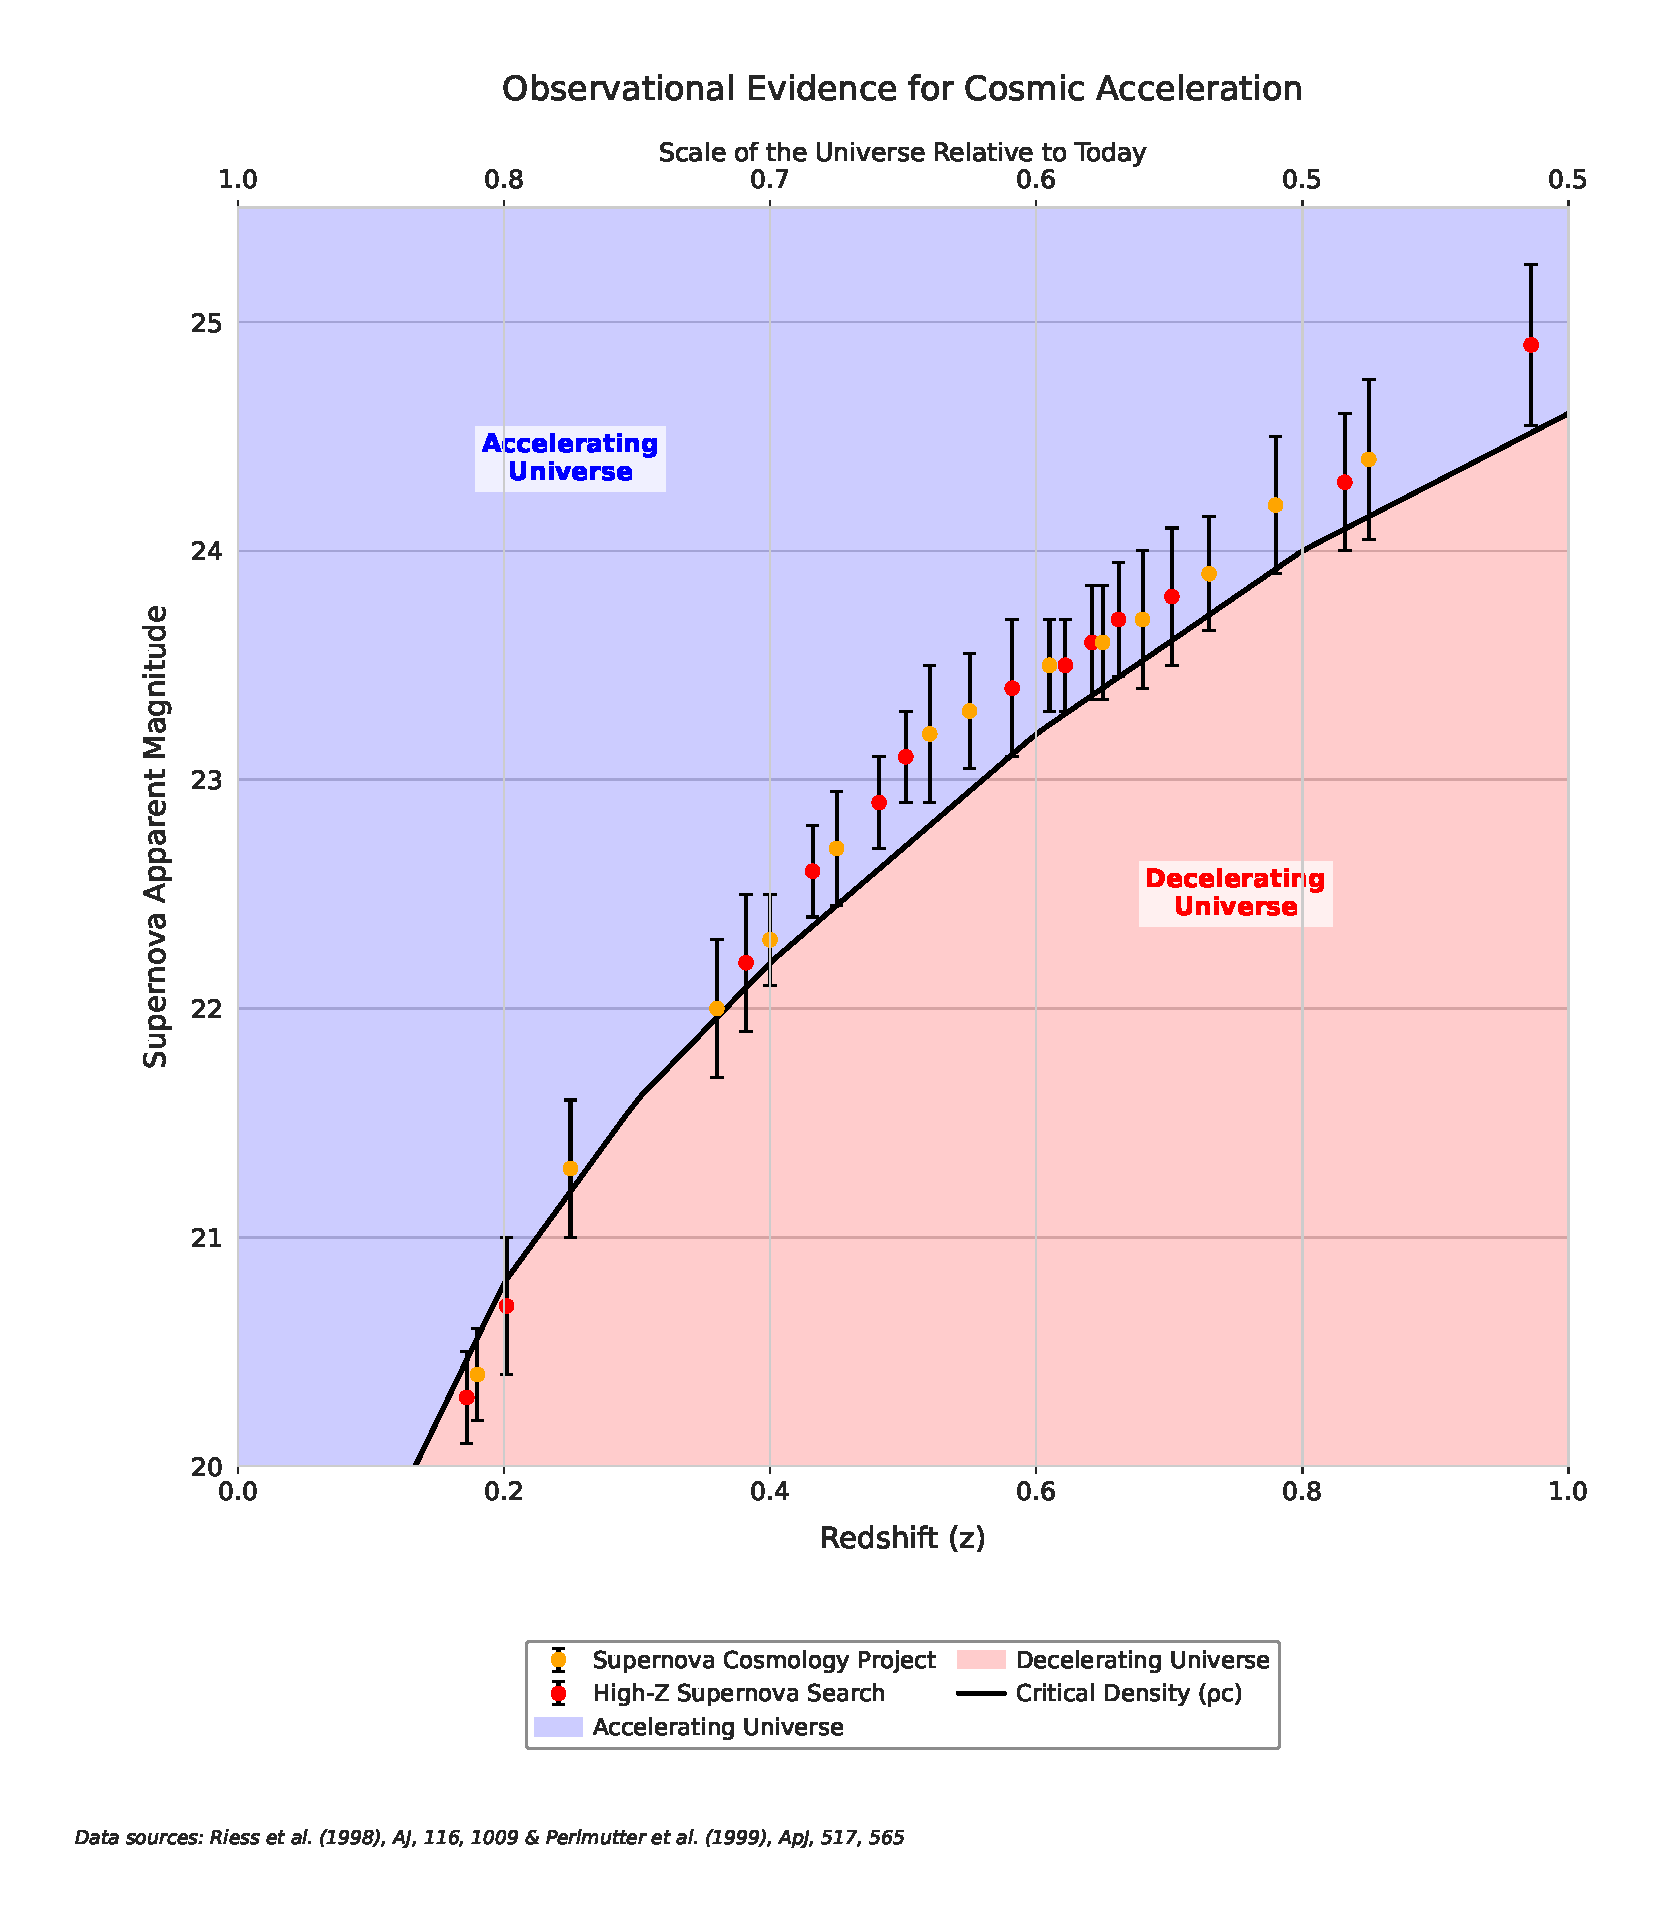
\includegraphics[width=\textwidth]{11_AcceleratingUniverse/hubble_graph_portrait.pdf}
}{}
}{%
    \IfFileExists{#1/imagefigure.tex}{%
      \imagefigure{
    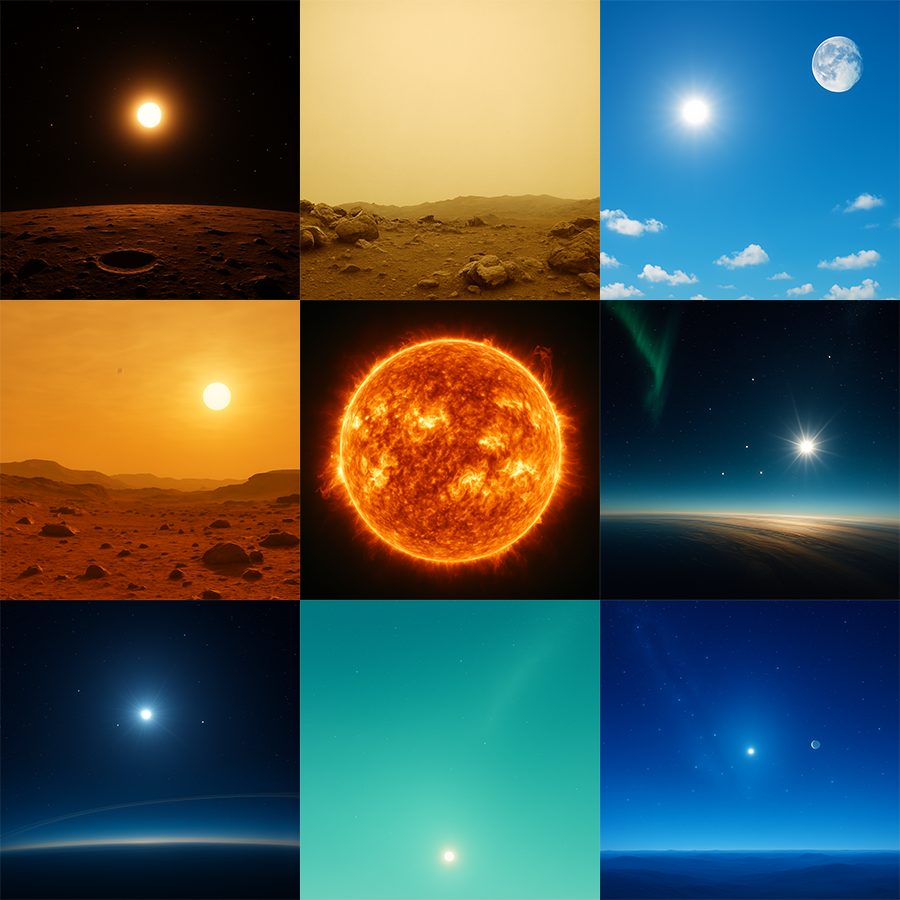
\includegraphics[width=0.8\textwidth]{27_PlanetarySkyColors/SKIES.png} 
}{
Nine simulated daytime skies from each planet in the Solar System, arranged heliocentrically around the Sun in a 3×3 grid. The rows (left to right, top to bottom) correspond to: Mercury, Venus, Earth; Mars, Sun, Jupiter; Saturn, Uranus, Neptune. Each panel reflects sky color, atmospheric scattering, and visible celestial features such as moons, rings, and the Sun’s apparent size, as modeled for surface or high-atmosphere observation.
}

      % IMAGE is full-page, do NOT add "End of Chapter" after this
    }{%
    % If none of the above exist, then maybe insert End of Chapter
    \checkoddpage
    \ifoddpage
      \clearpage
      \centeredfullpage{End of Chapter}{Turn to the next story.}
    \else
      % Already at end of sixth page
    \fi
    }}}}


}

\newsavebox{\SideTextBox}
\newenvironment{SideNotePage}[2] % #1 = side text, #2 = image path
{%
  \newpage
  \thispagestyle{empty}
  \begingroup
  \pagecolor{lavender}
  \vspace*{-0.3cm}%
  \noindent
  \fcolorbox{white}{white}{%
    \begin{minipage}{\dimexpr\linewidth-2\fboxsep-2\fboxrule}
    \noindent
    \begin{tabular}{@{}p{1.85in}@{\hspace{0.1in}}!{\color{lightgray}\vrule width 0.4pt}@{\hspace{0.1in}}p{4.22in}@{}}
    \begin{minipage}[t]{1.85in}
    \footnotesize
    #1
    \end{minipage}
    &
    \centering
    \vspace{0pt}\includegraphics[width=4.22in,height=9.2in,keepaspectratio]{#2}
    \end{tabular}%
    \end{minipage}
  }%
}
{%
  \endgroup
  \clearpage
  \pagecolor{white}
}





% Ensure technical environment doesn't break across pages
\AtEndEnvironment{technical}{\nopagebreak[4]}


% Enable only specific chapters
\begin{comment}

\def\showBanachTarskiParadox{}
\def\showGoldRelativity{}
\def\showArrowTheoremTopology{}
\def\showCircleWheel{}
\def\showEMFieldsEnergyFlow{}
\def\showAcceleratingUniverse{}
\def\showBilliardsConicsPorism{}
\def\showGravityTimeDilation{}
\def\showFourDSpacetime{}
\def\showBoundedPrimeGaps{}
\def\showSolarFusionQuantumTunneling{}
\def\showHatMonotile{}
\def\showSpeculativeExecutionAttacks{}
\def\showGSMEncryptionOrder{}

\def\showPoissonsSpot{}
\def\showTopologicalInsulators{}
\def\showBlackHoleTimeDilationRedshift{}
\def\showCompactTwinParadox{}
\def\showTorricellisTrumpet{}
\def\showCosmicRayMuons{}
\def\showEnvelopeParadox{}
\def\showChineseRoomArgument{}
\def\showShoelaceKnotMechanics{}

\def\showSimpsonsParadox{}
\def\showZKProofs{}


\def\showExponentialMapsLieTheory{}
\def\showIncubationInequality{}
\def\showOsmosisDebye{}
\def\showBoltzmannBrain{}


\def\showQFTvGR{}
\def\showPlanetarySkyColors{}



\def\showTreesFromAir{}
\def\showDarkMatterEvidence{}
\def\showChristmasTruce{}


\def\showFireflyBioluminescence{}
\def\showIronMask{}
\def\showThreeBody{}
\def\showCreepers{}
\def\showSuperpermutationsBreakthrough{}

\def\showMaxwellDemon{}
\def\showWoodwardHoffmannRules{}
\def\showNegativeTemp{}
\def\showIceSlipperiness{}
\def\showNearFlatUniverse{}
\def\showBodySwappingPuzzle{}

\end{comment}



\def\showBanachTarskiParadox{}

% Title and author
\title{Unpopular Science}
\author{David H. Silver}
\date{\today}

\begin{document}

% Cover page
\begin{titlepage}

        
    \begin{tikzpicture}[remember picture, overlay]
        % Background image
        \node[anchor=center] at (current page.center) {
            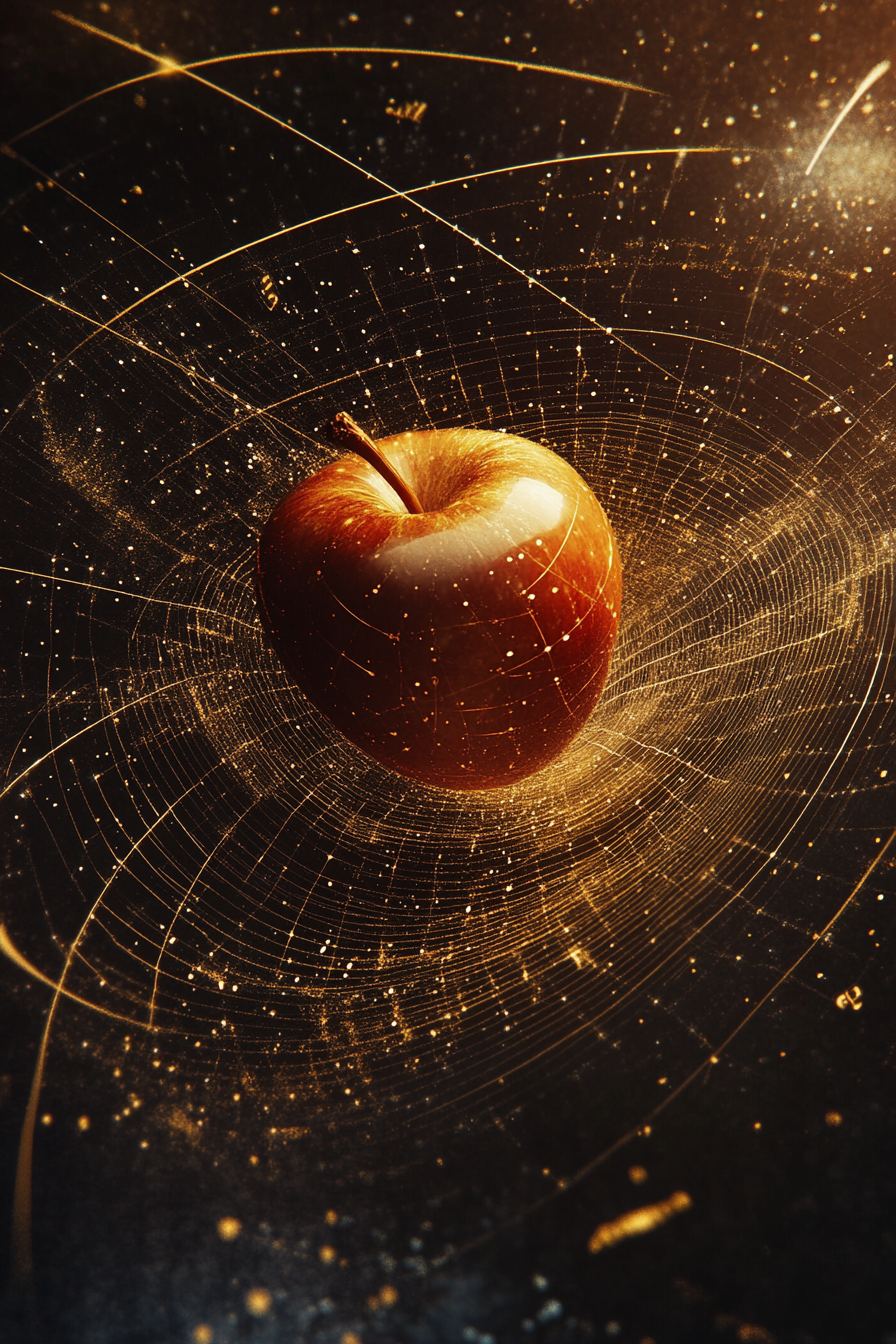
\includegraphics[width=\paperwidth,height=\paperheight]{MainBook_v120250308_014502/cover/locallysmooth_A_striking_book_cover_featuring_a_realistic_app_be06186c-f216-4d3a-8e43-cce948017fcb_1.png}
        };

        % Title
        \node[anchor=center, align=center] at ([yshift=-9cm]current page.center) {
            \fontsize{48}{52}\selectfont
            \bfseries\color{white}{Unpopular Science}\\
            \fontsize{48}{52}\selectfont
            \bfseries\color{red}{DRAFT}
        };


        % Author
        \node[anchor=center] at ([yshift=-11cm]current page.center) {
            \fontsize{18}{32}\selectfont
            \itshape\color{white} David H. Silver
        };
    \end{tikzpicture}
    \vfill
        
\end{titlepage}


% Introduction
\chapter*{Introduction}
\addcontentsline{toc}{chapter}{Introduction}
\begin{tcolorbox}[
    colback=white,
    colframe=gray!40,
    boxrule=0.5pt,
    arc=1mm,
    left=10pt,
    right=10pt,
    top=10pt,
    bottom=10pt,
    width=\textwidth,
    enlarge left by=0mm,
    sharp corners=south,
    breakable
]
\setlength{\parskip}{1em}

This book is not a popular science book. It is not a textbook. It is not an academic book. It is not even a chimera of the above.  

It does share some goals with the three: to inspire wonder (like a popular science book), to include some rigour (like textbooks), and to introduce readers to phenomena that might challenge their understanding (as academic works often achieve).

As with some combinations, like a sushi-pizza restaurant, it excels at none.  
You'll find that the main exposition is not long enough to really understand the subject, the technical part is either too abstract or too detailed to actually follow, and even though I claim rigour, mostly von Neumann's line that \textit{there's no sense in being precise when you don't know what you're talking about} fits too well.

But, if my plan works, you'll get the appetite to routinely leave this sushi-pizza diner and cross the street. Maybe to a fine-dining textbook because you're intrigued and want to solve it properly. Maybe to a street seller of roasted chestnuts, to browse Wikipedia or blogs and get more context for this absolutely fantastical world I'm trying to share with you.

All of the bits I'm sharing, except for a few that friends recommended, have a personal story. I remember how I learned about them, and I'm genuinely excited to write them down.  

I wish I could infect you with some of that excitement.

Here we go.
\end{tcolorbox}


\begin{tcolorbox}[
    colback=red!5,
    colframe=red!60!black,
    boxrule=1pt,
    arc=0.5mm,
    left=10pt,
    right=10pt,
    top=10pt,
    bottom=10pt,
    width=\textwidth,
    sharp corners=south,
    breakable,
    title=\textbf{DRAFT WARNING}
]
\setlength{\parskip}{1em}

This is a \textbf{very early draft}.\\
Parts of it are placeholders.\\
Some claims may be wrong.\\
Sections may vanish without notice.\\
Reader discretion is advised.

\begin{center}
{\addfontfeatures{LetterSpace=5.0}\scshape Manus adhuc in pulvere}\\
\textit{The hands are still in the dust.}
\end{center}

\end{tcolorbox}

\clearpage

\tableofcontents

% Prologue
\chapter*{Prologue}
\addcontentsline{toc}{chapter}{Prologue}
This book is about popular science — a return to the roots of scientific wonder, combining accessible explanations with the rigorous, often highly mathematical foundations behind them. Unlike much of contemporary science communication, which tends to oversimplify or sensationalize, this book seeks to highlight the beauty of science as it truly is: both elegant and complex. The focus here is on understanding, not just exposure.

Too often, modern science communicators rely on what I call a “laugh track” approach. They tell readers or viewers how they should feel about the material — “This is mind-blowing!” or “It’s unfathomable!” — instead of letting the wonder arise naturally from the ideas themselves. This technique, whether deliberate or not, can cheapen the experience, as though science requires a layer of manufactured excitement to be compelling. The reality is that science doesn’t need exaggeration. Its wonder is self-evident to those who take the time to explore it properly.

This book contains 50 stories, each structured to guide readers from the intuitive to the profound. Here’s how it will unfold:

\textbf{Historical Context} \ Each chapter begins with a concise historical background, offering insights into the people, circumstances, or discoveries that led to our understanding of the phenomenon. These stories ground the reader in the scientific journey, showing how human curiosity and perseverance have shaped our understanding of the world.

\textbf{Phenomenon Description} \ The phenomenon itself is then described in straightforward, down-to-earth terms. This section avoids sensational language, focusing instead on clear and accurate explanations. The aim is to make these concepts relatable while preserving their depth. Instead of declaring something “unbelievable,” we’ll show what makes it remarkable and allow the reader to appreciate it for themselves.

\textbf{Hardcore Analysis} \ For readers ready to dive deeper, the third section provides rigorous academic analysis. Here, the mathematical and technical underpinnings of the phenomenon are laid bare, complete with equations, references, and detailed derivations. This section is unapologetically tough, offering readers the tools to validate the claims, explore further, or simply appreciate the true complexity of the science.

While the Hardcore Analysis is not meant to be easily accessible — it is, in most cases, genuinely difficult to understand — it remains an essential part of each chapter. It exists not just for the few who can follow it in full, but for the integrity of the entire story. Much like the references section of a scientific article, it is not necessary to read in order to grasp the main ideas, but it is the shoulder on which the rest of the article stands. It provides scaffolding. It justifies the clarity above it. It reminds us that the simplified version is built on layers of rigor.

The goal of this structure is to respect the reader’s intelligence and curiosity. Whether discussing topological insulators, the mechanics of atomic clocks, or the subtleties of time dilation, the chapters will present science as it is: demanding, rewarding, and deeply inspiring.

This book seeks to counteract the trend of oversimplified science communication. Science is not a series of slogans or easy answers. Its complexity is not a flaw to be hidden but a feature to be celebrated. Understanding takes effort, but that effort transforms fleeting curiosity into lasting enlightenment.

If you’re ready to explore science in its full intellectual glory, I invite you to turn the page.



\begin{comment}
    \ifdefined\showIronMask
    \chapter[]{}
    \label{ch:}
    \inputstory{IronMask}
    \fi
\end{comment}

\ifdefined\showOsmosisDebye
\chapterwithsummary[ch:incubationinequality]{Concentrate on Osmosis}{Standard osmosis explanations based solely on water concentration gradients fail to account for measured flow rates that far exceed diffusion limits. The ratio of osmotic permeability to diffusive permeability (Pf/Pd) commonly exceeds 100 in biological systems with aquaporins, while purely diffusive transport would yield a ratio near 1. Mechanical explanations, notably Debye's model, attribute osmosis to pressure gradients arising from solute-membrane interactions rather than simple diffusion. When solutes are excluded by a semipermeable membrane, their momentum cannot transfer across the boundary, creating a localized pressure drop that drives water movement. This mechanistic framework better explains experimental observations, particularly the dramatic permeability differences between aquaporin channels and simple lipid bilayers.}
\inputstory{osmosis_Debye} %Approved
\fi


\ifdefined\showQFTvGR
\chapterwithsummary[ch:qftvsgr]{When Theories Collide}{General relativity and quantum field theory represent fundamentally incompatible frameworks for describing physical reality. GR portrays gravity as spacetime curvature — a geometric property emerging from mass-energy distribution — while QFT describes forces through particle exchange on a fixed background. This conceptual divide manifests in specific problems: the cosmological constant discrepancy (120 orders of magnitude between QFT vacuum energy predictions and observed values), the non-renormalizability of gravity (preventing standard quantum treatment), and the black hole information paradox (challenging quantum unitarity). These conflicts reveal the limits of our current understanding and motivate ongoing research into quantum gravity theories that might resolve these theoretical inconsistencies.}
\inputstory{qft_vs_gr} %Approved
\fi

\ifdefined\showTopologicalInsulators
\chapterwithsummary[ch:topologicalinsulators]{Edges of Tomorrow}{Topological insulators exhibit an unusual combination of properties: insulating in their bulk yet conducting electricity perfectly along surfaces or edges. This behavior originates from the material's topological structure, which guarantees protected conductive states resistant to scattering and imperfections. The mathematical concept of topology, concerning properties preserved under continuous deformation, manifests physically in these materials through robust edge states and quantized conductance. These properties arise from spin-orbit coupling and band inversion, creating boundary states that traverse the bulk energy gap and remain protected against perturbations that preserve time-reversal symmetry.}
\inputstory{TopologicalInsulators} %Approved
\fi


\ifdefined\showNegativeTemp
\chapterwithsummary[ch:negativetemperature]{Too Hot Or Too Cold}{Temperature fundamentally measures how entropy changes with energy (∂S/∂E), not merely kinetic activity. While unbounded systems like ideal gases can only reach positive temperatures, quantum systems with finite energy spectra reveal a complex structure. When energy addition increases disorder, temperature is positive; when maximum entropy is reached, temperature becomes infinite; further energy addition creates more ordered states with negative temperatures. These negative temperature states are not colder than absolute zero but hotter than infinity — they transfer energy to any positive-temperature system when brought into contact. This phenomenon occurs in systems like spin populations with population inversions, where the highest energy states are more populated than lower ones. The temperature scale forms a complete circle: 0+ → +∞ ≡ -∞ → 0-, with inverse temperature β = 1/(kBT) providing the more natural, continuous parameter.}
\inputstory{NegativeTemp} %Approved
\fi
    
\ifdefined\showExponentialMapsLieTheory
\chapterwithsummary[ch:exponentialmapslietheory]{Exponentially Generalizable}{The exponential function extends far beyond its familiar calculus definitions to form a unifying concept across mathematics. In various contexts: from formal power series to Lie theory, Riemannian geometry to sheaf theory — exponential maps share the fundamental property of transforming additive structures into multiplicative or compositional ones. These constructions are not coincidental; each maps linear or infinitesimal information to global or curved structures while preserving key relationships. Whether defined through power series, geodesics, or algebraic homomorphisms, exponential maps express how local linearity extends into global structure, demonstrating how mathematical abstractions reveal patterns across seemingly disparate domains.}
\inputstory{ExponentialMapsLieTheory} %Approved
\fi

\ifdefined\showBoltzmannBrain
\chapterwithsummary[ch:boltzmannbrain]{A Thought About Nothing}{The Boltzmann Brain paradox emerges from applying statistical physics to cosmology: in infinite time, random fluctuations in a high-entropy universe should produce isolated conscious entities far more frequently than entire ordered universes like ours. Mathematical analysis suggests a single brain with illusory memories requires vastly fewer unlikely coincidences than a genuine cosmic history. These hypothetical self-aware systems would possess false memories of existing in a structured world, despite being momentary arrangements with no causal history. The paradox creates cognitive instability — if observers are statistical fluctuations with false memories rather than evolved beings, the reliability of cosmological theories themselves becomes suspect.}
\inputstory{BoltzmannBrain} %Approved
\fi



\ifdefined\showBlackHoleTimeDilationRedshift
\chapterwithsummary[ch:blackholetimedilationredshift]{Everywhere at the End of Time}{General relativity predicts drastically different perspectives for observers watching an object fall into a black hole versus the falling object itself. External observers see the object progressively slow, redden, and dim as it approaches the event horizon, appearing to freeze at the boundary due to extreme gravitational time dilation. In contrast, the falling object experiences no unusual effects when crossing the event horizon, continuing inward without local indication of having passed this critical boundary. This disparity in observations illustrates how spacetime curvature alters the relationship between reference frames, arresting intuitions about simultaneity and time.}
\inputstory{BlackHoleTimeDilationRedshift} %Approved
\fi

\ifdefined\showMaxwellDemon
\chapterwithsummary[ch:maxwelldemon]{Entropy's Gatekeeper}{Maxwell's Demon, proposed in 1867, describes a thought experiment where a tiny being controls a door between two gas chambers, selectively allowing fast molecules into one chamber and slow ones into another. This sorting creates a temperature gradient from uniformity, seemingly decreasing entropy and violating the second law of thermodynamics. The resolution emerged through Landauer's principle (1961): the demon must erase information to continue sorting, and this erasure necessarily increases entropy by at least kB ln 2 per bit, offsetting the entropy reduction from sorting. This connection between information processing and thermodynamics reveals that information has physical embodiment with real thermodynamic consequences. The paradox remains relevant in quantum contexts, where measurement actively changes systems and quantum statistics alter the sorting possibilities.}
\inputstory{MaxwellDemon} %Approved
\fi
    
\ifdefined\showCompactTwinParadox
\chapterwithsummary[ch:compacttwinparadox]{A Circle of Time}{In a cylindrical universe with compact spatial dimensions, twins can separate and reunite without acceleration, with one traveling around the circumference while the other remains stationary. Despite neither experiencing acceleration, they age differently upon reunion, creating a variant of the famous paradox for special relativity. In non-orientable topologies like Klein bottle universes, travelers can additionally experience reversal of chirality. Even a thoroughly non-dextrocardic explorer might come back from a cosmic stroll with his heart on the right side, no trauma needed.}
\inputstory{CompactTwinParadox} %Approved
\fi


\ifdefined\showShoelaceKnotMechanics
\chapterwithsummary[ch:shoelaceknotmechanics]{Knot Your Average Shoelace}{The tendency for shoelaces to spontaneously untie stems from the interplay between knot topology and applied forces during walking. The common "granny knot" is topologically less stable than the "square knot," despite their superficial similarity. Which knot forms depends on the orientation of the initial crossing relative to subsequent looping motions. Walking generates cyclic impact forces and inertial oscillations that gradually loosen the weaker knot structure by allowing slack to propagate through the system. And perhaps — just perhaps — that's why children are convinced their parents tie better knots: a shoelace secured by Grandma, viewed from a frame with reversed chirality, might literally hold tighter.}
\inputstory{ShoelaceKnotMechanics} %Approved
\fi


\ifdefined\showIncubationInequality
\chapterwithsummary[ch:incubationinequality]{Gaussian Correlation Inequality}{The Gaussian Correlation Inequality states that for two convex, symmetric sets in high-dimensional space, the probability of a Gaussian-distributed random point landing in both regions simultaneously is at least the product of the individual probabilities. This relationship, connecting geometric structure to probabilistic behavior, remained unproven for over fifty years despite verification in special cases. In 2014, Thomas Royen, a retired statistics professor from a university of applied sciences, resolved the conjecture using elementary tools: Laplace transforms and properties of gamma distributions.}
\inputstory{IncubationInequality} %Approved
\fi

\ifdefined\showGoldRelativity
\chapterwithsummary[ch:goldrelativity]{All That Gold Glitters}{The yellow color of gold requires relativistic quantum mechanics to explain, unlike silver's silvery appearance. Electrons in gold atoms reach 58\% of light speed, causing the 6s orbital to contract and the 5d orbital to expand. This shifts absorption to blue wavelengths, resulting in the reflection of yellow-red light. Similar relativistic effects explain mercury's liquid state and platinum's white appearance. These everyday properties demonstrate how modern physics manifests in macroscopic observations.}
\inputstory{GoldRelativity} %Approved
\fi

\ifdefined\showCircleWheel
\chapterwithsummary[ch:circlewheel]{A Full Circle of PIE}{The terms "wheel" and "cycle" (but not circle!) derive from Proto-Indo-European *kʷékʷlos despite their phonetic dissimilarity in modern languages. Regular sound shifts transformed this root differently in Germanic and Hellenic branches through documented phonological processes. These linguistic patterns preserve evidence of Bronze Age terminology and illustrate consistent patterns of language change. Comparative methods identify these transformations through sound correspondences across Indo-European languages.} %Approved
\inputstory{CircleWheel} %Approved
\fi

\ifdefined\showPhotosynthesisQuantumEfficiency
\chapter[Illuminating Life: The Science of Photosynthesis]{Illuminating Life: The Science of Photosynthesis}
\label{ch:photosynthesis-quantumefficiency}
\inputstory{Photosynthesis_QuantumEfficiency}
\fi

\ifdefined\showIronMask
\chapterwithsummary[ch:ironmask]{The Mask of Administrative Silence}{The prisoner known as "Eustache Dauger" remained in state custody for thirty-four years (1669-1703) under extraordinary protocols of secrecy. His confinement spanned four locations under the continuous supervision of a single jailer, Bénigne Dauvergne de Saint-Mars. Official correspondence reveals exceptional measures: a specially constructed cell with sound isolation, strict limitations on communication, and a requirement to wear a black velvet mask (not iron) when visible to anyone outside Saint-Mars's control. The prisoner served as valet to another detainee at Pignerol before eventual transfer to the Bastille, where he died and was buried under the alias "Marchioly." No court proceedings, charges, or legal classification appear in records, and following his death, all his possessions and cell surfaces were destroyed — creating a case distinguished not by the known elements but by systematic erasure of official identity.}
\inputstory{IronMask} %Approved
\fi


\ifdefined\showCreepers
\chapterwithsummary[ch:minecraftcreeper]{Creeping Bug}{The Creeper, Minecraft's iconic explosive enemy, originated from a simple programming error when developer Markus Persson accidentally swapped height and length values while modeling a pig. Rather than discarding the tall, narrow result, Persson repurposed the glitch, adding a leaf-block texture, downturned mouth, and silent approach behavior culminating in detonation. The mob's mechanics were assembled from existing code: pathfinding logic, recycled textures, and the game's block destruction system. Its distinctive threat comes from simple parameters — entering "swell" state when within 2.5 blocks of a player and resetting when beyond 6 blocks — combined with silent movement that creates asymmetric encounters.}
\inputstory{MinecraftCreeper} %Approved
\fi

    
\ifdefined\showTreesFromAir
\chapterwithsummary[ch:treesfromair]{From Air to Arbor}{Trees derive their mass primarily from atmospheric carbon dioxide rather than soil — contrary to intuitive belief. Through photosynthesis, plants convert this gaseous carbon into solid form, with approximately 95\% of a tree's dry mass originating from air. Carbon (45-50\%), oxygen (40-45\%), and hydrogen (6\%) constitute the vast majority of wood structure, while soil minerals contribute only 1-5\%. This process transforms diffuse atmospheric gases into the solid structure of forests, demonstrating that substantial physical objects can be essentially materialized air fixed by solar energy.}
\inputstory{TreesFromAir} %Approved
\fi

\ifdefined\showBanachTarskiParadox
\chapterwithsummary[ch:banachtarskiparadox]{An Axiom of Your Choice}{The Banach-Tarski paradox demonstrates how a sphere can be decomposed and reassembled into two identical spheres under certain axiomatic frameworks. This counterintuitive result depends on the Axiom of Choice and non-measurable sets, which allow infinite sets to behave in ways that differs from physical intuition about volume conservation. While physically impossible, the paradox illuminates how mathematical foundations shape concepts and highlights the distinction between mathematical existence and physical realizability.}
\inputstory{BanachTarskiParadox} %Approved
\fi

\ifdefined\showEMFieldsEnergyFlow
\chapterwithsummary[ch:energytransmission]{Think Outside the Wire}{Electrical energy travels primarily through electromagnetic fields surrounding conductors, not through the movement of electrons in wires. While electrons drift at millimeters per second, energy transfer occurs near light speed through the Poynting vector (S = E × B), which describes energy flow perpendicular to both electric and magnetic fields. This field-based transmission explains why circuits respond almost instantly despite slow electron movement, challenging the common misconception that electricity flows like water through pipes. Rather, the phenomenon resembles waves propagating across water's surface, where energy travels through the medium while the particles themselves undergo minimal displacement.}
\inputstory{EMFieldsEnergyFlow} %Approved
\fi


\ifdefined\showThreeBody
\chapterwithsummary[ch:threebody]{Chaotic Neutrality}{Deterministic systems with fixed rules can exhibit chaotic behavior, where minuscule differences in initial conditions lead to drastically different outcomes over time. The double pendulum, three-body gravitational problem, and irregular billiard tables exemplify this phenomenon despite having few components and simple governing equations. Counterintuitively, billions of times more complex physical systems like falling objects often display predictable behavior. This is because dissipative effects — friction, air resistance, and internal vibration — continuously suppress perturbations.}
\inputstory{three_body}  %Approved
\fi


\ifdefined\showZKProofs
\chapterwithsummary[ch:zkproofs]{The Proof, The Whole Proof, and Nothing But The Proof }{Zero-knowledge proofs enable verifying the truth of a statement without revealing any information beyond its validity. These cryptographic protocols satisfy three properties: completeness (valid statements can be proven), soundness (false statements cannot be proven), and zero-knowledge (the proof reveals nothing about the statement except its truth). The mechanisms rely on cryptographic commitments, challenge-response interactions, or probabilistic verification that make it computationally infeasible to succeed without knowing the secret. Applications include authentication without password transmission, privacy-preserving transactions, and confidential verification of regulatory compliance.} %Approved
\inputstory{ZKProofs}
\fi



\ifdefined\showSuperpermutationsBreakthrough
\chapterwithsummary[ch:superpermutationsbreakthrough]{Superanonymous}{A significant breakthrough in the superpermutation problem originated from an unlikely source: an anonymous 4chan post responding to a question about anime episode viewing orders. Superpermutations are strings containing every possible ordering of n symbols as substrings. For years, mathematicians believed the minimal length followed the pattern of factorial sums observed in small cases. The anonymous poster derived a rigorous lower bound: L(n) ≥ n! + (n-1)! + (n-2)! + n - 3, modeling the problem as path optimization through a permutation graph. This proof remained obscure until 2018 when mathematician Robin Houston rediscovered it, leading to the disproof of the long-standing conjecture and establishing new bounds on this combinatorial problem — with the original derivation still officially credited to "Anonymous 4chan Poster."}
\inputstory{SuperpermutationsBreakthrough} %Approved
\fi

\ifdefined\showGSMEncryptionOrder
\chapterwithsummary[ch:gsmencryptionorder]{You Would Like to Order First}{GSM mobile communications used the A5/1 encryption algorithm to protect call privacy, but its implementation revealed how engineering decisions can undermine cryptographic security. The system encrypted data by XORing it with a keystream generated from a 64-bit key, but weaknesses emerged from the protocol's structure rather than the algorithm itself. By encrypting signaling data before voice data, the system exposed predictable message patterns that allowed attackers to recover encryption keys through known-plaintext attacks.}
\inputstory{GSMEncryptionOrder} %Approved
\fi

\ifdefined\showArrowTheoremTopology
\chapterwithsummary[ch:arrowtheoremtopology]{\textit{Real} Democracy Has Never Been Tried}{Arrow's Impossibility Theorem proves that no voting system can simultaneously satisfy all seemingly reasonable criteria for fair collective decision-making. The theorem demonstrates that any method for aggregating ranked preferences must violate at least one of several axioms: non-dictatorship, Pareto efficiency, independence of irrelevant alternatives, or transitivity.} %Approved
\inputstory{ArrowTheoremTopology}
\fi


\ifdefined\showPlanetarySkyColors
\chapterwithsummary[ch:planetaryskycolors]{A Spectrum of Skies}{The colors observed in astronomical objects originate from defined physical interactions between light and matter. Earth's blue sky results from Rayleigh scattering, where atmospheric molecules preferentially scatter shorter wavelengths. This principle extends across astronomy, where spectral modifications encode properties like temperature, composition, and motion. Stars emit thermal radiation with characteristic spectra determined by temperature — hotter stars appear blue, cooler stars red. Planets derive colors from reflection, absorption, and scattering processes in their atmospheres and surfaces. Nebulae display colors through emission from ionized gas, reflection of starlight by dust, or absorption creating dark silhouettes.}  %Approved
\inputstory{PlanetarySkyColors}
\fi

\ifdefined\showSolarFusionQuantumTunneling
\chapterwithsummary[ch:solarfusionquantumtunneling]{The Tunnel at the Beginning of Light}{Solar fusion proceeds despite temperatures insufficient for classical nuclear reactions because quantum tunneling enables protons to penetrate the Coulomb barrier with non-zero probability. At the Sun's core temperature of 15 million Kelvin, the average proton possesses only about 1/20 the energy classically required to overcome electromagnetic repulsion between positively charged nuclei. Quantum mechanics allows particles to "tunnel" through energy barriers they cannot surmount classically, with probability decreasing exponentially with barrier height and width. This tunneling effect, combined with the enormous number of interaction attempts in the solar plasma, sustains the precise fusion rate necessary for stellar stability over billions of years.}
\inputstory{SolarFusionQuantumTunneling} %Approved
\fi

\ifdefined\showBilliardsConicsPorism
\chapterwithsummary[ch:billiardsconicsporism]{A Complex (Projective) Billiard Game}{Poncelet's Porism describes an unexpected property of billiard trajectories between two nested ellipses: if one path returns to its starting point after a finite number of bounces, then all starting points generate periodic trajectories with the same number of bounces. This geometric result connects to elliptic curves in number theory and measure-preserving dynamical systems. The theorem exemplifies how problems in distinct mathematical fields — from billiards to Gelfand's question about decimal digits — reduce to the same structure when expressed through appropriate frameworks.} 
\inputstory{BilliardsConicsPorism} %Approved
\fi

\ifdefined\showGravityTimeDilation
\chapterwithsummary[ch:gravitytimedilation]{The Apple Falls the Shortest Path from the Tree}{General relativity reveals gravity as a manifestation of spacetime curvature where time and space metrics are affected by massive objects. As opposed to the depiction of gravity as bending space, like the rubber sheet visualizations, it is actually the gradient in time's passage that creates what appears as gravitational attraction, guiding objects toward regions of slower time. This perspective resolves the apparent force of gravity as a natural consequence of objects following the simplest path through curved time, rather than being pulled by an invisible force.}
\inputstory{GravityTimeDilation} %Approved
\fi



\ifdefined\showEnvelopeParadox
\chapterwithsummary[ch:envelopeparadox]{The Better Envelope}{The Envelope Paradox presents two envelopes where one contains twice the money of the other. After selecting one envelope, seemingly valid probabilistic reasoning suggests an expected gain by switching (averaging 1/x with 2x), regardless of which envelope was initially chosen. This symmetric conclusion creates a logical inconsistency since perpetual switching cannot be optimal. The paradox arises from improper application of expected value calculations to scenarios with unbounded distributions or when conditional probabilities are not properly accounted for. Resolving the paradox requires distinguishing between known values and variables, recognizing when probability distributions are ill-defined, and understanding the limitations of expected value calculations with potentially infinite quantities.}
\inputstory{EnvelopeParadox} %Approved
\fi

\ifdefined\showSpeculativeExecutionAttacks
\chapterwithsummary[ch:speculativeexecutionattacks]{A Leaky Crystal Ball}{Speculative execution optimizes performance by executing instructions before knowing if they're needed, leaving microarchitectural traces in cache memory even when results are discarded. Attacks like Meltdown and Spectre exploit this by constructing code sequences where a secret value determines which memory addresses are accessed during speculation. By measuring which addresses load quickly afterward (indicating they were cached), attackers can determine if specific bits were 0 or 1. This technique allows secrets to be extracted across privilege boundaries despite never appearing in architectural state.}
\inputstory{SpeculativeExecutionAttacks}%Approved
\fi




\ifdefined\showBoundedPrimeGaps
\chapterwithsummary[ch:boundedprimegaps]{70-Million Steps for Primes, one giant leap for mankind}{In 2013, an unaffiliated Yitang Zhang proved there exists a finite bound B (initially 70,000,000) such that infinitely many prime pairs differ by at most B. While prime gaps can grow arbitrarily large, this breakthrough showed they cannot consistently drift apart without bound. The Polymath8 collaboration subsequently reduced this bound to a few hundred. Zhang's approach combined distribution properties of primes in arithmetic progressions with an advanced sieving technique, resolving a fundamental question about number patterns while falling short of proving the Twin Prime Conjecture that infinitely many primes differ by exactly 2.} 
\inputstory{BoundedPrimeGaps} %Approved
\fi

\ifdefined\showAcceleratingUniverse
\chapterwithsummary[ch:acceleratinguniverse]{Dark Energies Are Pushing Us Apart}{Observations of distant supernovae in the 1990s revealed that the universe's expansion is accelerating, contradicting earlier models that predicted gravity would slow cosmic expansion. This acceleration requires dark energy, an unknown component comprising about 70\% of the universe's energy density. Dark energy counteracts gravity at cosmological scales, manifesting as either a cosmological constant in Einstein's equations or a dynamical field.}
\inputstory{AcceleratingUniverse} %Approved
\fi

\ifdefined\showIceSlipperiness
\chapterwithsummary[ch:iceslipperiness]{Ice, Ice, Maybe}{Ice's exceptional slipperiness results primarily from a quasi-liquid layer (QLL) of disordered water molecules at its surface rather than from commonly assumed mechanisms. While pressure melting and frictional heating contribute under specific conditions, neither explains ice's slickness at rest or across wide temperature ranges. Surface molecules, having fewer hydrogen bonds than those in the interior crystal lattice, form a nanometer-thick disordered layer that functions as a molecular lubricant even well below freezing. Counterintuitively, ice is most slippery around -7°C rather than at 0°C, as the QLL is sufficiently mobile at this temperature while the underlying ice remains hard enough to resist deformation.}
\inputstory{IceSlipperiness} %Approved
\fi

\ifdefined\showChristmasTruce
\chapterwithsummary[ch:christmastruce1914]{A Pause in the Pattern}{The 1914 Christmas Truce demonstrated how environmental conditions, shared cultural rituals, and mutual recognition briefly transformed conflict into spontaneous cooperation along the Western Front. Soldiers from opposing armies halted fighting to exchange gifts, sing carols, and fraternize in no man's land. This phenomenon emerged from multiple converging factors: the physical hardship of trench warfare, recognition of shared traditions and circumstances, the recent onset of war before dehumanization had fully taken hold, and implicit mutual understanding of common suffering.}
\inputstory{ChristmasTruce1914} %Approved
\fi


\ifdefined\showWoodwardHoffmannRules
\chapterwithsummary[ch:woodwardhoffmannrules]{Symmetry's Chemical Logic}{The Woodward-Hoffmann rules establish how mathematical symmetry conservation governs chemical reaction pathways at the quantum level. In pericyclic reactions, the symmetry properties of molecular orbitals — represented by wave functions with specific nodal patterns analogous to trigonometric functions — must be conserved throughout the reaction coordinate. This conservation requirement creates selection rules that determine allowed stereochemical outcomes. The symmetry constraints differ fundamentally between thermal and photochemical conditions, as light excitation inverts the orbital symmetry relationships, thereby enabling reaction pathways forbidden under thermal conditions and vice versa.}
\inputstory{WoodwardHoffmannRules} %Approved
\fi



\ifdefined\showTorricellisTrumpet
\chapterwithsummary[ch:torricellistrumpet]{Hey Mr. Trumpet Man, Paint a Horn for Me}{Torricelli's Trumpet, generated by rotating y=1/x around the x-axis for x≥1, illustrates how geometric intuition breaks down with infinite objects. This solid extends infinitely yet contains a finite volume of exactly π cubic units, as proven through integration. Simultaneously, its surface area is infinite, creating the apparent paradox that the trumpet could be filled with a finite amount of paint yet never painted completely. The divergence occurs because volume scales with the square of radius while surface area scales linearly with radius as x approaches infinity.}
\inputstory{TorricellisTrumpet} %Approved
\fi

\ifdefined\showQuantumSubspaceAngles
\chapter[Angles of Connection: Geometry in Quantum Subspaces]{Angles of Connection: Geometry in Quantum Subspaces}
\label{ch:quantumsubspaceangles}
\inputstory{QuantumSubspaceAngles}
\fi

\ifdefined\showBodySwappingPuzzle
\chapterwithsummary[ch:bodyswappingpuzzle]{The Futurama Theorem}{The body swapping puzzle explores a mathematical problem that gained prominence through the animated series Futurama: when multiple individuals swap minds, can everyone return to their original bodies if no pair can swap directly more than once? This question connects to permutation group theory, where mind swaps represent cycles in permutation notation. The Futurama Theorem, formally known as Keeler's Theorem after writer Ken Keeler, proves that regardless of how complex the initial swapping arrangement, adding two fresh bodies allows any permutation to be sorted with only pairwise swaps.}
\inputstory{BodySwappingPuzzle} %Approved
\fi



\ifdefined\showHatMonotile
\chapterwithsummary[ch:hatmonotile]{The Plane Hat of Einstein}{In 2023, the "hat" tile discovery resolved the long-standing Einstein problem in tiling theory. This 13-sided polygon covers the plane completely while guaranteeing no pattern repetition, enforcing aperiodicity through geometry alone with just the tile and its mirror image. The breakthrough began with David Smith, an amateur mathematician and tiling enthusiast who noticed unusual behaviors during hands-on experimentation. Working with professional mathematicians, Smith helped develop and verify the formal proofs.}
\inputstory{HatMonotile} %Approved
\fi

\ifdefined\showCosmicRayMuons
\chapterwithsummary[ch:cosmicraymuons]{Consider the Muon's PoV}{Muons created by cosmic rays colliding with the upper atmosphere provide direct evidence for time dilation. With a rest-frame lifetime of approximately 2.2 microseconds and traveling close to light speed, classical physics predicts these particles should decay before reaching Earth's surface. Instead, detectors routinely observe muons at sea level. Special relativity explains this observation: from Earth's reference frame, the muons' time runs slower by a factor of γ (approximately 10-50 depending on energy), extending their lifetime enough to reach ground level. From the muon's perspective, relativistic length contraction reduces the distance traveled.}
\inputstory{CosmicRayMuons} %Approved
\fi

\ifdefined\showChineseRoomArgument
\chapterwithsummary[ch:chineseroomargument]{Capish, Comprehendes, Computes?}{John Searle's Chinese Room thought experiment challenges computational theories of mind by proposing a scenario where someone manipulates Chinese symbols according to explicit rules without understanding the language. This person could produce appropriate responses to Chinese input, passing a linguistic Turing test, yet possess no comprehension of the conversation's meaning. The argument distinguishes syntax (symbol manipulation) from semantics (understanding), suggesting that digital computers executing algorithms necessarily operate only at the syntactic level. This distinction questions whether systems like large language models truly understand language or merely simulate understanding through statistical pattern recognition, highlighting differences between rule-following behavior and genuine comprehension.}
\inputstory{ChineseRoomArgument}  %Approved
\fi


\ifdefined\showDarkMatterEvidence
\chapterwithsummary[ch:darkmatterevidence]{The Invisible Scaffold}{Dark matter's existence is inferred through multiple independent lines of evidence spanning different cosmic scales. Galaxy rotation curves remain flat far beyond visible matter, indicating extended gravitational influence. Galaxy clusters contain hot gas whose temperature and confinement require gravitational potentials deeper than visible matter can provide. Gravitational lensing reveals mass distributions exceeding luminous components, particularly in systems like the Bullet Cluster where dark and visible matter separate during collisions. Cosmic web structure formation requires gravitational scaffolding predating visible matter to develop within observed timeframes. The cosmic microwave background's fluctuation patterns indicate that ordinary matter comprises only 15\% of the total matter content needed to match observations, with the remainder consisting of non-baryonic material already present before photon-matter decoupling.}
\inputstory{DarkMatterEvidence} %Approved
\fi

\ifdefined\showNearFlatUniverse
\chapterwithsummary[ch:nearflatuniverse]{Infinite Yet Born}{The universe appears flat to within 0.4\% precision according to cosmic microwave background measurements. This flatness, described by the Lambda-CDM model, indicates that space follows Euclidean geometry even across vast cosmological distances. The universe may be spatially infinite while having a finite age of 13.8 billion years. This implication comes from the Big Bang model: an expansion of intergalactic space rather than an explosion within pre-existing space. If space was already infinite at the beginning, it expanded uniformly from every point. No center to the universe!}
\inputstory{NearFlatUniverse} %Approved
\fi

\ifdefined\showPoissonsSpot
\chapterwithsummary[ch:poissonsspot]{Right on Spot}{Poisson's spot (also called the Arago spot) demonstrates wave diffraction through the unexpected appearance of a bright point at the center of a circular object's shadow. When Augustin-Jean Fresnel proposed light as a wave phenomenon in 1818, Siméon Poisson derived this counterintuitive prediction to disprove the theory. According to wave principles, light diffracting around a circular obstacle creates constructive interference exactly at the center point where waves from all directions arrive in phase. François Arago's experimental confirmation of this bright central spot, which had seemed absurd under particle theory, provided compelling evidence for the wave nature of light, transforming what was intended as a refutation into definitive validation.}
\inputstory{PoissonsSpot} %Approved
\fi


\ifdefined\showSimpsonsParadox
\chapterwithsummary[ch:simpsonsparadox]{Divide and Conquer}{Simpson's Paradox occurs when a statistical trend present in separate groups reverses when the groups are combined. This effect emerges from unequal group sizes or hidden confounding variables that distribute non-uniformly across the data. For example, a treatment might show positive effects in both male and female subgroups yet appear harmful in the aggregate population if the treatment is disproportionately given to patients with more severe conditions and males and females differ in average severity. The paradox demonstrates that causal inference requires accounting for relevant stratifying variables and careful consideration of the causal structure rather than relying solely on raw correlations.}
\inputstory{SimpsonsParadox}  %Approved
\fi

\ifdefined\showFourDSpacetime
\chapterwithsummary[ch:4dspacetime]{Put on Your 4D Glasses}{Four dimensions appear repeatedly across physics and mathematics as a critical boundary for stable structures. In three spatial dimensions plus time, inverse-square laws permit stable orbits, quantum field theories remain renormalizable, gauge interactions systematically cancel anomalies, and exotic smooth structures emerge uniquely. This dimensionality enables crucial mathematical frameworks including quaternions, instantons, and black hole uniqueness theorems. Lower dimensions lack sufficient complexity for certain structures, while higher dimensions introduce instabilities and weaken constraints that produce the observable patterns of physical law.}
\inputstory{FourDSpacetime}  %Approved
\fi

\ifdefined\showFireflyBioluminescence
\chapterwithsummary[ch:fireflybioluminescence]{Let There Be Bioluminescence}{Fireflies produce light through a precise biochemical reaction where luciferase enzymes catalyze the oxidation of luciferin in specialized abdominal photocytes. This process converts chemical energy to light with remarkable efficiency — over 80\% compared to an incandescent bulb's 5\% — creating "cold light" with minimal heat production. Fireflies control flash patterns by regulating oxygen flow through tracheal networks, producing species-specific signals that prevent cross-species mating attempts. The light emission peaks in the yellow-green spectrum (560-590 nm), optimized for visibility in low-light conditions. Reflective layers of uric acid crystals direct photons outward, enhancing visibility. This natural system demonstrates the convergence of genetics, biochemistry, cellular biology, and quantum physics, where electron transitions between energy levels determine the wavelength of emitted photons.}
\inputstory{FireflyBioluminescence}
\fi


\begin{comment}
    \ifdefined\showTheMissingMiddle
\chapter[Lost in the Gap: The Disappearing Middle Class]{Lost in the Gap: The Disappearing Middle Class}
\label{ch:themissingmiddle}
\inputstory{TheMissingMiddle}
\fi



\ifdefined\showPhysicalConstraintsComputing
\chapter[Physics of Computing: Beyond the Code]{Physics of Computing: Beyond the Code}
\label{ch:physicalconstraintscomputing}
\inputstory{PhysicalConstraintsComputing}
\fi


\ifdefined\showSexContinuum
\chapter[Beyond the Binary: The Spectrum of Biological Sex]{Beyond the Binary: The Spectrum of Biological Sex}
\label{ch:sexcontinuum}
\inputstory{SexContinuum}
\fi


\ifdefined\showCliffYoungShuffle
\chapter[Endurance Unleashed: The Power of a Steady Shuffle]{Endurance Unleashed: The Power of a Steady Shuffle}
\label{ch:cliffyoungshuffle}
\inputstory{CliffYoungShuffle}
\fi
\ifdefined\showMatterAntimatterAsymmetry
\chapter[Why Matter Matters: The Mystery of Antimatter Asymmetry]{Why Matter Matters: The Mystery of Antimatter Asymmetry}
\label{ch:matterantimatterasymmetry}
\inputstory{MatterAntimatterAsymmetry}
\fi


\ifdefined\showObserverDependentVacuum
\chapter[Perspectives of the Quantum Vacuum]{Perspectives of the Quantum Vacuum}
\label{ch:observerdependentvacuum}
\inputstory{ObserverDependentVacuum}
\fi


\ifdefined\showSolarNeutrinos
\chapter[Neutrinos: The Invisible Messengers of Solar Fusion]{Neutrinos: The Invisible Messengers of Solar Fusion}
\label{ch:solarneutrinos}
\inputstory{SolarNeutrinos}
\fi

\ifdefined\showExpanderGraphsPSL2q
\chapter[Expander Graphs: Sparse Connections, Strong Bonds]{Expander Graphs: Sparse Connections, Strong Bonds}
\label{ch:expandergraphspsl2q}
\inputstory{ExpanderGraphsPSL2q}
\fi

\ifdefined\showGreatDivergenceDebate
\chapter[Unraveling the Great Divergence: Europe's Economic Ascent]{Unraveling the Great Divergence: Europe's Economic Ascent}
\label{ch:greatdivergencedebate}
\inputstory{GreatDivergenceDebate}
\fi

\ifdefined\showGameTheoryCooperation
\chapter[The Power of Cooperation: Evolution's Collaborative Advantage]{The Power of Cooperation: Evolution's Collaborative Advantage}
\label{ch:gametheorycooperation}
\inputstory{GameTheoryCooperation}
\fi

\ifdefined\showEigenvectorCentralityInPolitics
\chapter[Unveiling Influence: The Power of Eigenvector Centrality in Networks]{Unveiling Influence: The Power of Eigenvector Centrality in Networks}
\label{ch:eigenvectorcentralityinpolitics}
\inputstory{EigenvectorCentralityInPolitics}
\fi

\ifdefined\showBoomerangFlight
\chapter[Boomerangs: The Aerodynamics of Returning Flight]{Boomerangs: The Aerodynamics of Returning Flight}
\label{ch:boomerangflight}
\inputstory{BoomerangFlight}
\fi

\end{comment}

\end{document}

